\hypertarget{02b_secenekler_hukuk}{%
\chapter{Faz 2B --- Seçenekler, bitiş durumu ve hukuki yol haritası}\label{02b_secenekler_hukuk}}

\textbf{Durum:} Faz 2 / 9 tamamlandı (18 Ekim 2026); DEVAM bekleniyor. Birinci kısım: \belgebag{02a_politika_uzayi}{}{\kod{02a\_\allowbreak{}politika\_\allowbreak{}uzayi.\allowbreak{}md}}. Önceki faz: \belgebag{01_teshis}{}{\kod{01\_\allowbreak{}teshis.\allowbreak{}md}}. Defter: \belgebag{defter}{}{\kod{defter.\allowbreak{}md}}.

\textbf{Bu belge ne yapıyor?} Faz 2A, Türkiye'nin kendi araçlarının sınırlarını çizdi. Bu belge dört şey yapıyor:

\begin{itemize}
\tightlist
\item
  dış rejim seçeneklerini sayısal olarak karşılaştırıyor (§1--§3);
\item
  iki takvim için bitiş durumunu ve geçiş sırasını öneriyor (§4);
\item
  AB, DTÖ ve Türk iç hukuku açısından adım adım yol haritasını çiziyor (§5);
\item
  olasılıkları, kapıları ve riskleri güncelliyor (§6--§7).
\end{itemize}

Kanıt etiketleri ve güven düzeyleri 02a'daki gibi.

\textbf{Veri ve kod.}

\begingroup\gbtablo\small

\begin{longtable}[]{@{}
  >{\raggedright\arraybackslash}p{(\columnwidth - 4\tabcolsep) * \real{0.2390}}
  >{\raggedright\arraybackslash}p{(\columnwidth - 4\tabcolsep) * \real{0.4926}}
  >{\raggedright\arraybackslash}p{(\columnwidth - 4\tabcolsep) * \real{0.2684}}@{}}
\toprule\noalign{}
\begin{minipage}[b]{\linewidth}\raggedright
\textbf{Betik}
\end{minipage} & \begin{minipage}[b]{\linewidth}\raggedright
\textbf{İçerik}
\end{minipage} & \begin{minipage}[b]{\linewidth}\raggedright
\textbf{Ana kaynak}
\end{minipage} \\
\midrule\noalign{}
\endhead
\bottomrule\noalign{}
\endlastfoot
\kod{kod/\allowbreak{}f2f\_\allowbreak{}cekim\_\allowbreak{}modeli.\allowbreak{}py} & Yapısal çekim modeli (PPML): GB'nin ve AB STA'larının (derin, temel) ticaret etkisi; S2, S3 ve S4 senaryoları; genel denge modülü & CEPII Gravity V202211, BACI 2024, DESTA v2.3, UN AMA \\
\kod{kod/\allowbreak{}f2e\_\allowbreak{}s4\_\allowbreak{}aktif.\allowbreak{}py} & Aktif S4 paketleri ve S3'te menşe maliyetinin TÜFE etkisi & 02a \\
\kod{kod/\allowbreak{}f2c\_\allowbreak{}vergi\_\allowbreak{}takasi.\allowbreak{}py}, \kod{kod/\allowbreak{}f2d\_\allowbreak{}s4\_\allowbreak{}net\_\allowbreak{}istihdam.\allowbreak{}py} & Vergi takası; net istihdam & 02a \\
\end{longtable}

\endgroup

Hukuki bulgular Faz 2'nin AB hukuku ve DTÖ hukuku araştırma notlarından alındı. \etiketV{} etiketli olanlar birincil metinden okundu: Ankara Anlaşması, Katma Protokol, 1/95, ABİDA md. 207/217/218, Mercosur, Şili ve Meksika kararları, TCA, revize PEM, NANDO, DTÖ Analitik Endeksi.

\begin{center}\rule{0.5\linewidth}{0.5pt}\end{center}

\hypertarget{02b_secenekler_hukuk-faz-2bnin-10-ana-bulgusu}{%
\section{Faz 2B'nin 10 ana bulgusu}\label{02b_secenekler_hukuk-faz-2bnin-10-ana-bulgusu}}

\begin{enumerate}
\def\labelenumi{\arabic{enumi}.}
\tightlist
\item
  \textbf{Anlaşmasız çıkışın (S4) ticaret kaybı sağlam ve büyük.}

  \begin{itemize}
  \tightlist
  \item
    Türkiye'nin AB'ye ihracatı −\%19 (GE; \%90 GA −\%32 ile −\%5). Kısmi denge −\%22; Faz 0 tarife duvarı hesabı −\%15 ile −\%33.
  \item
    Toplam ihracat −\%6,2; reel GSYH −\%0,43 (GA −\%0,73 ile −\%0,10).
  \item
    Bu bir alt sınır, çünkü 1971'den beri süren sanayi tercihleri modelde ikili sabit etkiye düşüyor.
  \item
    \etiketT{} Güven: Orta.
  \end{itemize}
\item
  \textbf{Derin STA'nın (S2) maliyeti belirsiz ve muhtemelen küçük.}

  \begin{itemize}
  \tightlist
  \item
    Merkez tahmin: AB'ye ihracatta −\%11, GSYH'de −\%0,22. İkisinin de GA'sı sıfırı içeriyor.
  \item
    Dünya Bankası (2014): −\%3 ile −\%7.
  \item
    \etiketT{} Güven: Düşük--Orta.
  \end{itemize}
\item
  \textbf{Temel STA'nın (S3) sonucu tasarıma bağlı.}

  \begin{itemize}
  \tightlist
  \item
    Aralık −\%18 ile +\%1.
  \item
    Türkiye--BK STA'sı (2021) sıfır tarifeyi ve AB girdisiyle kümülasyonu korudu. GB'den STA'ya geçişte ticaret kaybı istatistiksel olarak sıfır çıktı.
  \item
    Ders: menşe protokolü müzakerenin en kritik başlığıdır.
  \item
    \etiketT{} Güven: Düşük--Orta.
  \end{itemize}
\item
  \textbf{Hiçbir çıkış seçeneği bütün kısıtları kendiliğinden sağlamıyor.}

  \begin{itemize}
  \tightlist
  \item
    TÜFE ve mali kısıtlar her seçenekte tasarımla karşılanabiliyor.
  \item
    İstihdam kısıtı S2'de bile risk altında: ≈ −33 bin, GA sıfırı içeriyor. Sınıf düzeyinde uyum ve destek paketi (Faz 3--5) her seçenekte gerekli.
  \item
    \etiketT{} Güven: Düşük--Orta.
  \end{itemize}
\item
  \textbf{Önerilen bitiş durumu S2 (DCFTA), 2030--2031.}

  \begin{itemize}
  \tightlist
  \item
    İçerik: sanayide sıfır tarife, PEM ve tam kümülasyon, öncelikli sektörlerde ACAA, hizmetler, kamu alımı, karayolu, eşit rekabet koşulları; Türkiye'nin tarife özerkliği ve kendi STA ağı.
  \item
    Ara durum S3 (md. 207 ITA). Geçiş R7 (dondurma). Geri dönüş planı aktif S4.
  \item
    \etiketH{} Güven: Orta.
  \end{itemize}
\item
  \textbf{İki takvim.}

  \begin{itemize}
  \tightlist
  \item
    \textbf{T2029:} ITA 1.1.2029'da geçici uygulamada. Bunun için AB müzakere yetkisinin Eylül 2027'ye kadar verilmesi gerekiyor.
  \item
    \textbf{T2028:} yalnızca çıkış kararı ve dondurma (geçiş dönemi); ITA 2029--2030'da.
  \item
    Ortaklık Konseyi kararı GB'yi kaldıramaz. GB'nin hukuken sona ermesi ITA'nın ``GB hükümleri etkisiz kalır'' maddesiyle olur (AB--Şili md. 33.11 emsali).
  \item
    Öneri: ekonomik ve hukuki çıkış T2029; T2028 gerekiyorsa çıkış kararı ve geçiş başlangıcı.
  \item
    \etiketV{}/\etiketH{} Güven: Orta.
  \end{itemize}
\item
  \textbf{AB tarafında yol var: nitelikli çoğunluk.}

  \begin{itemize}
  \tightlist
  \item
    Dondurma kararında AB pozisyonu (md. 218(9) + 207(4); C-81/13), ITA yetkisi ve imzası nitelikli çoğunlukla alınıyor. Bu, Faz 0'daki oybirliği varsayımının düzeltmesi.
  \item
    Yunanistan ve GKRY'nin hukuki vetosu yok; siyasi vetoları var.
  \item
    Belirleyici başkentler Berlin ve Roma. Mercosur'da beş üye devletin karşı oyuna rağmen karar çıktı.
  \item
    Risk: Divan'ın Görüş 1/26'sı ITA ayrımını daraltabilir.
  \item
    \etiketV{} Güven: Orta--Yüksek.
  \end{itemize}
\item
  \textbf{Onaylanmış kuruluş uçurumu gerçek.}

  \begin{itemize}
  \tightlist
  \item
    NANDO'da 95 Türk kaydı var; ≈81'i yürürlükte.
  \item
    Süreklilik hükmü olmadan Türk sertifikaları çıkış günü AB'de geçersiz olur (İngiltere 2020, İsviçre 2021 dersleri).
  \item
    Dondurma kararına ve ITA'ya ``büyükbaba'' hükmü konmalı.
  \item
    \etiketV{} Güven: Yüksek.
  \end{itemize}
\item
  \textbf{Olasılıklar güncellendi (hasmane AB, kapılar işletilmeden).}

  \begin{itemize}
  \tightlist
  \item
    T2028'de anlaşmasız çıkış \%55--68; T2029'da \%30--50.
  \item
    Kapılar işletilirse bu olasılığın çoğu erteleme anlamına gelir; çıkış yönü değişmez, tarih değişir.
  \item
    \etiketH{} Güven: Düşük.
  \end{itemize}
\item
  \textbf{En büyük risk tarife değil, kur.}

  \begin{itemize}
  \tightlist
  \item
    \%10'luk bir değer kaybı TÜFE'ye ≈+250 bp ekler; bu, aktif S4'ün tarife kanalının 30--80 katı.
  \item
    Çıkışın kurallı, önceden ilan edilmiş ve anlaşmaya dayalı olması tarife tasarımından daha önemli.
  \item
    Makro çerçeve Faz 6'da.
  \item
    \etiketV{}/\etiketH{} Güven: Orta.
  \end{itemize}
\end{enumerate}

\begin{center}\rule{0.5\linewidth}{0.5pt}\end{center}

\hypertarget{02b_secenekler_hukuk-1-seuxe7eneklerin-tanux131mux131}{%
\section{1. Seçeneklerin tanımı}\label{02b_secenekler_hukuk-1-seuxe7eneklerin-tanux131mux131}}

\begin{landscape}

\begingroup\gbtablo\footnotesize

\begin{longtable}[]{@{}
  >{\raggedright\arraybackslash}p{(\columnwidth - 18\tabcolsep) * \real{0.0975}}
  >{\raggedright\arraybackslash}p{(\columnwidth - 18\tabcolsep) * \real{0.1058}}
  >{\raggedright\arraybackslash}p{(\columnwidth - 18\tabcolsep) * \real{0.0879}}
  >{\raggedright\arraybackslash}p{(\columnwidth - 18\tabcolsep) * \real{0.1133}}
  >{\raggedright\arraybackslash}p{(\columnwidth - 18\tabcolsep) * \real{0.0887}}
  >{\raggedright\arraybackslash}p{(\columnwidth - 18\tabcolsep) * \real{0.1271}}
  >{\raggedright\arraybackslash}p{(\columnwidth - 18\tabcolsep) * \real{0.0976}}
  >{\raggedright\arraybackslash}p{(\columnwidth - 18\tabcolsep) * \real{0.1009}}
  >{\raggedright\arraybackslash}p{(\columnwidth - 18\tabcolsep) * \real{0.1032}}
  >{\raggedright\arraybackslash}p{(\columnwidth - 18\tabcolsep) * \real{0.0780}}@{}}
\toprule\noalign{}
\begin{minipage}[b]{\linewidth}\raggedright
\textbf{Seçenek}
\end{minipage} & \begin{minipage}[b]{\linewidth}\raggedright
\textbf{TR → AB tarife}
\end{minipage} & \begin{minipage}[b]{\linewidth}\raggedright
\textbf{AB → TR tarife}
\end{minipage} & \begin{minipage}[b]{\linewidth}\raggedright
\textbf{Türkiye'nin üçüncü ülkelere tarifesi ve STA'ları}
\end{minipage} & \begin{minipage}[b]{\linewidth}\raggedright
\textbf{Menşe}
\end{minipage} & \begin{minipage}[b]{\linewidth}\raggedright
\textbf{Uyum değerlendirmesi}
\end{minipage} & \begin{minipage}[b]{\linewidth}\raggedright
\textbf{Hizmet, kamu alımı, hareketlilik}
\end{minipage} & \begin{minipage}[b]{\linewidth}\raggedright
\textbf{Eşit rekabet koşulları ve uyuşmazlık}
\end{minipage} & \begin{minipage}[b]{\linewidth}\raggedright
\textbf{AB'de hukuki yol}
\end{minipage} & \begin{minipage}[b]{\linewidth}\raggedright
\textbf{Müzakere süresi (emsal)}
\end{minipage} \\
\midrule\noalign{}
\endhead
\bottomrule\noalign{}
\endlastfoot
\textbf{S0} Statüko GB & 0 (sanayi, İTÜ) & 0 & OGT'ye bağlı; paralel STA & Gerekmiyor (A.TR) & 1/95 md. 8--10; Türk onaylanmış kuruluşları geçerli & GB dışında & Ortaklık Konseyi; zayıf & --- & --- \\
\textbf{S1} Modernize GB & 0; tarım ve hizmetler genişler & 0 & OGT; Türkiye'nin STA sürecine katılımı (``Türkiye maddesi'') & A.TR & Aynı & Hizmet ve kamu alımı açılır & Güçlü uyuşmazlık çözümü & Ortaklık Konseyi kararı + karma anlaşma; Konsey yetkisi 10 yıldır yok & 3--5 yıl \\
\textbf{S2} DCFTA & 0 (menşe şartıyla) & 0 (menşe şartıyla) & \textbf{Özerk}; kendi STA ağı & Revize PEM; tam kümülasyon & ACAA veya MRA & Hizmet, kamu alımı, karayolu ve vize faslı & Sübvansiyon denetimi, yeniden dengeleme, tahkim & Md. 207 veya 217 & 3--6 yıl; 2030 sonrası \\
\textbf{S3} Temel STA (md. 207 ITA) & 0 (menşe şartıyla) & 0 (menşe şartıyla) & Özerk & Revize PEM ve çapraz kümülasyon & ACAA yok; \textbf{onaylanmış kuruluş geçiş hükmü şart} & Sınırlı & Hafif; tahkim & Md. 207 (nitelikli çoğunluk) + AP onayı; geçici uygulama mümkün & ≈12 ay (TCA 10 ay) \\
\textbf{R7} Dondurma (geçici anlaşma) & 0 & 0 & OGT dondurma süresince sürer & A.TR & Statü sürer & --- & Ortaklık Konseyi & Ortaklık Konseyi kararı; AB pozisyonu md. 218(9), nitelikli çoğunluk & 6--9 ay \\
\textbf{S4-aktif} Anlaşmasız çıkış + tek taraflı paket & AB MFN (\%5,85; €5,5 mlr) & MFN; İGV rejimi c2; girdide sıfır; vergi takası & Özerk & Gerekmiyor (MFN) & Türk sertifikaları AB'de geçersiz & --- & DTÖ & --- & --- \\
\textbf{S5} Gerilim & AB MFN + ticaret savunmasında sertleşme & Aynı & Özerk & --- & Geçersiz & --- & AB karşı önlemleri & --- & --- \\
\end{longtable}

\endgroup

\end{landscape}

\emph{Not:} S3'ün hukuki aracı R8'dir: AB'nin tek başına yetkili olduğu md. 207 Geçici Ticaret Anlaşması. Bu anlaşma GB hükümlerini ``etkisiz kılar'' (§5.1). S2, S3'ün üzerine kurulan karma bir anlaşma olarak sonra gelebilir.

\begin{center}\rule{0.5\linewidth}{0.5pt}\end{center}

\hypertarget{02b_secenekler_hukuk-2-karux15fux131laux15ftux131rma-matrisi}{%
\section{2. Karşılaştırma matrisi}\label{02b_secenekler_hukuk-2-karux15fux131laux15ftux131rma-matrisi}}

\hypertarget{02b_secenekler_hukuk-21-ticaret-etkisi-uxe7ekim-modeli}{%
\subsection{2.1 Ticaret etkisi: çekim modeli}\label{02b_secenekler_hukuk-21-ticaret-etkisi-uxe7ekim-modeli}}

\textbf{Yöntem} (\kod{kod/\allowbreak{}f2f\_\allowbreak{}cekim\_\allowbreak{}modeli.\allowbreak{}py}):

\begin{itemize}
\tightlist
\item
  Model: yapısal çekim modeli, PPML (Yotov vd. 2016).
\item
  Sabit etkiler: ihracatçı-yıl, ithalatçı-yıl ve yönlü ikili.
\item
  Örnek: CEPII Gravity, 1988--2020, 4 yıllık aralık, ilk 150 ekonomi; 2024'e BACI ile uzatma.
\item
  Kuklalar:

  \begin{itemize}
  \tightlist
  \item
    GB'nin iki yönü: Türkiye → AB ve AB → Türkiye;
  \item
    AB'nin derin STA'ları (Kore, CETA, Japonya, Vietnam, DCFTA'lar);
  \item
    AB'nin temel STA'ları (Avrupa-Akdeniz anlaşmaları, Meksika 2000, Şili 2003);
  \item
    kontroller.
  \end{itemize}
\item
  Senaryo etkisi: S0'a göre \% değişim = exp(β\_senaryo − β\_GB) − 1; S4'te β = 0.
\item
  Kısmi denge: çok taraflı direnç terimleri sabit. Genel denge modülü ayrıca raporlandı.
\end{itemize}

\Needspace{7\baselineskip}

\textbf{Tablo 2.1 --- Ana katsayılar (M1, PPML; parantez içinde küme-sağlam standart hata)}

\nopagebreak[4]

\begingroup\gbtablo\small

\begin{longtable}[]{@{}
  >{\raggedright\arraybackslash}p{(\columnwidth - 6\tabcolsep) * \real{0.1393}}
  >{\raggedleft\arraybackslash}p{(\columnwidth - 6\tabcolsep) * \real{0.1218}}
  >{\raggedleft\arraybackslash}p{(\columnwidth - 6\tabcolsep) * \real{0.1109}}
  >{\raggedright\arraybackslash}p{(\columnwidth - 6\tabcolsep) * \real{0.6280}}@{}}
\toprule\noalign{}
\begin{minipage}[b]{\linewidth}\raggedright
\textbf{Değişken}
\end{minipage} & \begin{minipage}[b]{\linewidth}\raggedleft
\textbf{Katsayı}
\end{minipage} & \begin{minipage}[b]{\linewidth}\raggedleft
\textbf{Yüzde etki}
\end{minipage} & \begin{minipage}[b]{\linewidth}\raggedright
\textbf{Sağlamlık aralığı (19 spesifikasyon)}
\end{minipage} \\
\midrule\noalign{}
\endhead
\bottomrule\noalign{}
\endlastfoot
GB: Türkiye → AB & +0,246 (0,130) & +\%28 & +0,04 ile +0,36. 1996 öncesi ortaklık rejimine göre artış: AB sanayide 1971'den beri Türk mallarına tarife uygulamıyordu \\
GB: AB → Türkiye & +0,142 (0,120) & +\%15 & −0,08 ile +0,44 \\
AB'nin derin STA'ları & +0,100 (0,039) & +\%11 & +0,01 ile +0,13; 2020'ye ve uzaklık × yıl kontrolüne duyarlı \\
AB'nin temel STA'ları & −0,167 (0,056) & −\%15 & −0,21 ile −0,07. \textbf{Kullanılamaz:} anlaşma öncesinde anlamlı bir eğilim var (4 yıl önceki öncül katsayı −0,19, p \textless{} 0,01). Avrupa-Akdeniz ortaklarının anlaşmadan önce de tercihli erişimi vardı. Bu yüzden S3 için Türkiye'nin kendi GB ↔ STA geçişleri kullanıldı \\
\end{longtable}

\endgroup

\Needspace{7\baselineskip}

\textbf{Tablo 2.1b --- Senaryolar: S0'a (GB) göre Türkiye'nin AB'ye ihracatı ve diğer göstergeler}

\nopagebreak[4]

\begingroup\gbtablo\footnotesize

\begin{longtable}[]{@{}
  >{\raggedright\arraybackslash}p{(\columnwidth - 10\tabcolsep) * \real{0.2817}}
  >{\raggedleft\arraybackslash}p{(\columnwidth - 10\tabcolsep) * \real{0.1404}}
  >{\raggedleft\arraybackslash}p{(\columnwidth - 10\tabcolsep) * \real{0.1417}}
  >{\raggedleft\arraybackslash}p{(\columnwidth - 10\tabcolsep) * \real{0.1456}}
  >{\raggedleft\arraybackslash}p{(\columnwidth - 10\tabcolsep) * \real{0.1642}}
  >{\raggedleft\arraybackslash}p{(\columnwidth - 10\tabcolsep) * \real{0.1265}}@{}}
\toprule\noalign{}
\begin{minipage}[b]{\linewidth}\raggedright
\end{minipage} & \begin{minipage}[b]{\linewidth}\raggedleft
\textbf{Kısmi denge (M1; \%90 GA)}
\end{minipage} & \begin{minipage}[b]{\linewidth}\raggedleft
\textbf{Genel denge (σ = 7; \%90 GA)}
\end{minipage} & \begin{minipage}[b]{\linewidth}\raggedleft
\textbf{Türkiye toplam ihracatı (GE)}
\end{minipage} & \begin{minipage}[b]{\linewidth}\raggedleft
\textbf{Türkiye reel GSYH, refah vekili (GE)}
\end{minipage} & \begin{minipage}[b]{\linewidth}\raggedleft
\textbf{AB reel GSYH (GE)}
\end{minipage} \\
\midrule\noalign{}
\endhead
\bottomrule\noalign{}
\endlastfoot
\textbf{S2} DCFTA & −\%13,6 (−30,5 ile +7,4) & −\%11,1 (−26,7 ile +6,1) & −\%3,3 (−8,3 ile +2,1) & −\%0,22 (−0,56 ile +0,19) & −\%0,01 \\
\textbf{S3, ihtiyatlı} (Türkiye'nin aday ülkelerle STA'sından GB'ye geçiş, 2004/2007/2013) & −\%22,0 (−35,1 ile −6,4) & −\%18,2 (−31,1 ile −3,4) & −\%5,3 (−10,6 ile +1,3) & −\%0,35 (−0,75 ile +0,15) & −\%0,02 \\
\textbf{S3, iyimser} (Türkiye--BK'nin GB'den STA'ya geçişi, 2021) & +\%0,3 (−9,2 ile +10,9) & +\%1,4 (−6,7 ile +10,5) & +\%1,1 (−1,7 ile +4,5) & +\%0,10 (−0,11 ile +0,35) & 0 \\
\textbf{S4} & −\%21,8 (−36,9 ile −3,2) & −\%18,9 (−32,4 ile −4,6) & −\%6,2 (−10,6 ile −1,5) & −\%0,43 (−0,73 ile −0,10); σ = 5'te −\%0,63 & −\%0,03 \\
Karşılaştırma: Faz 0 tarife duvarı (S4, kısmi denge, σ = 3 / 5 / 8) & −\%15 / −\%23 / −\%33 & & & & \\
Karşılaştırma: Dünya Bankası (2014), GB yerine menşe kurallı STA & −\%3,0 ile −\%7,2 & & & & \\
\end{longtable}

\endgroup

\emph{Kaynak ve etiketler:}

\begin{itemize}
\item
  \etiketT{} \kod{veri/\allowbreak{}politika\_\allowbreak{}cekim\_\allowbreak{}katsayilar.\allowbreak{}csv}, \kod{veri/\allowbreak{}politika\_\allowbreak{}cekim\_\allowbreak{}senaryolar.\allowbreak{}csv}.
\item
  Örnek: 150 ekonomi; 1988--2020, 4 yıllık aralık. N = 185.003, 21.480 çift.
\item
  Tahminde ülke içi ticaret yok (USITC ITPD-E erişilemedi). Etkiler üçüncü ülkelerle ticarete göredir; yaratma ve saptırmayı birlikte içerir.
\item
  GE: 2019 kesiti; ülke içi satışlar UN AMA katma değerinden türetildi; kesin şapka cebiri; \%90 GA 1.000 çekilişli parametrik bootstrap.
\item
  \textbf{Etkinin zaman yolu (M2).} GB etkisi hemen ortaya çıkıyor, sonra sönümleniyor:

  \begin{itemize}
  \tightlist
  \item
    Türkiye → AB: 0--3 yılda +\%44, 4--7 yılda +\%25, 8--11 yılda +\%34, 12+ yılda +\%21 (anlamsız).
  \item
    AB → Türkiye: +\%55, +\%40, +\%16, −\%3.
  \end{itemize}

  Derin STA etkisi ilk 8 yılda ≈+\%9.
\item
  \textbf{Kırılganlık.} Derin STA katsayısı 2020'ye (2020 hariç 0,012; BACI 2024 uzatmasıyla yine 0,099) ve uzaklık × yıl kontrolüne (0,014) duyarlı.

  \begin{itemize}
  \tightlist
  \item
    Yalnızca DCFTA'lar alındığında (M6; Rusya ile ticaret kırılması kontrol edilerek) S2: Türkiye → AB −\%9,8 (−31 ile +18).
  \item
    GB katsayısı veri kaynağına ve aralığa duyarlı: 5 yıllık aralıkta 1995 taban yılı zaten ``tedavi edilmiş'', çünkü Türkiye 1993--95'te tarifelerini önceden indirdi.
  \end{itemize}
\item
  \textbf{Literatürle uyum.} Aytuğ vd. (2017) +\%38 buluyor; bizim ilk on yıl tahminimiz +\%34--44. Dünya Bankası (2014) ikili etkiyi anlamsız buluyor; bu, AB → Türkiye sonucumuzla ve 5 yıllık ve BACI varyantlarıyla uyumlu. Dursun (2023) sönümlenmeyi buluyor; bizde de var.
\item
  Güven: Orta (S4), Düşük--Orta (S2, S3).
\end{itemize}

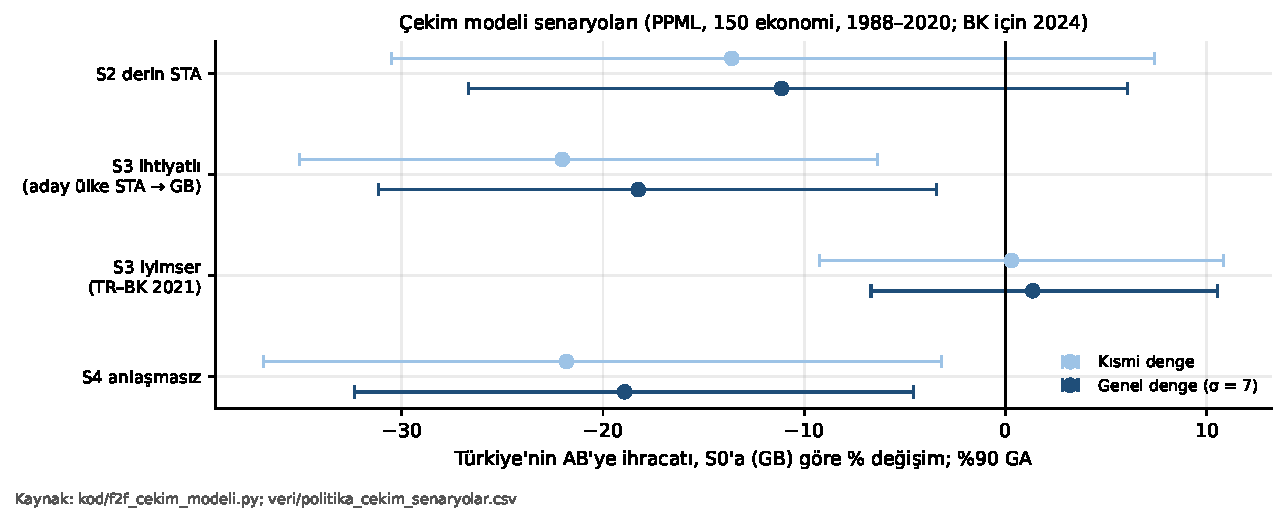
\includegraphics[width=1\textwidth,height=\textheight]{sekiller/f2_cekim_senaryo.pdf}

\emph{Şekil 2B.1 --- Çekim modeli: S2, S3 ve S4'ün Türkiye'nin AB'ye ihracatına etkisi (S0'a göre; \%90 GA)}

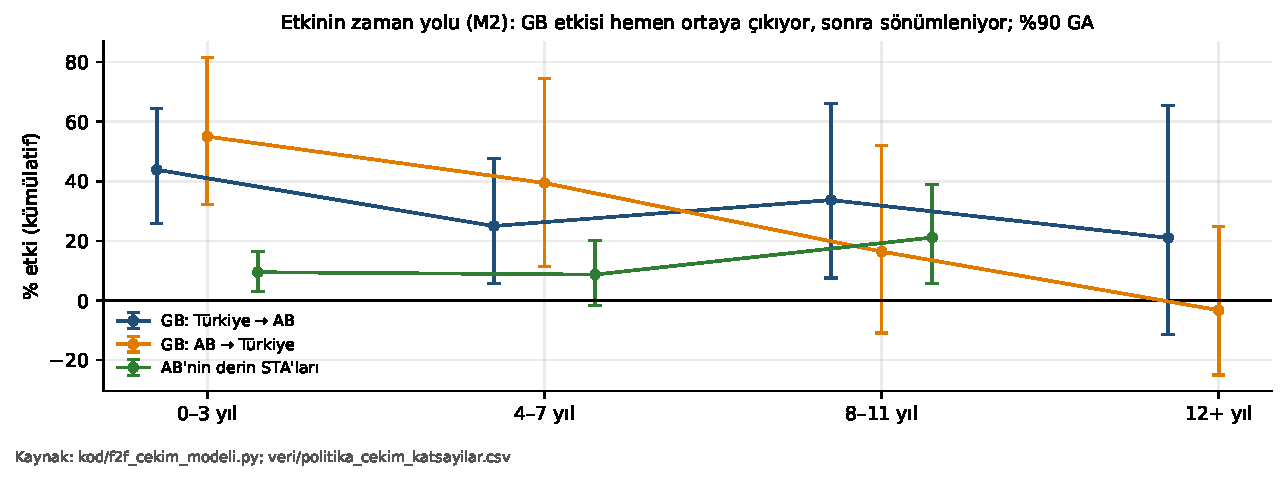
\includegraphics[width=1\textwidth,height=\textheight]{sekiller/f2_cekim_zaman_yolu.pdf}

\emph{Şekil 2B.2 --- GB ve AB'nin derin STA'larının ticaret etkisinin zaman yolu (M2; \%90 GA)}

\textbf{Okuma.}

\begin{enumerate}
\def\labelenumi{\arabic{enumi}.}
\tightlist
\item
  \textbf{S4'ün ticaret kaybı sağlam.}

  \begin{itemize}
  \tightlist
  \item
    Kısmi denge, genel denge ve tarife duvarı hesabı aynı bölgeye düşüyor: Türkiye'nin AB'ye ihracatında −\%19 ile −\%23.
  \item
    Bu bir alt sınır, çünkü 1971'den beri süren tercihler ve Türkiye'nin 1993--95 tarife indirimleri ikili sabit etkide kalıyor.
  \item
    Reel GSYH kaybının GA'sı sıfırı dışlıyor.
  \item
    AB → Türkiye için tarife duvarı çapraz kontrolü: İGV hariç −\%12 ile −\%27, İGV dahil −\%22 ile −\%42.
  \end{itemize}
\item
  \textbf{S2'nin kaybı belirsiz.} Merkez tahmin −\%11, ama GA sıfırı içeriyor.

  \begin{itemize}
  \tightlist
  \item
    GB katsayısı muhtemelen 1996'da kalkan tekstil kotalarının etkisini de içeriyor \etiketH{}. Bir STA bu kotaları geri getirmez; bu yüzden S2'nin kaybı muhtemelen merkez tahminden küçük.
  \item
    GB etkisi zamanla sönümleniyor. Uzun vadede (12+ yıl, M2) S2'nin S0'a göre etkisi ≈0 (+\%0,1; GA −28 ile +40).
  \item
    Dünya Bankası'nın −\%3 ile −\%7 aralığı bu okumayla uyumlu.
  \end{itemize}
\item
  \textbf{S3'ün sonucu tasarıma bağlı.}

  \begin{itemize}
  \tightlist
  \item
    İhtiyatlı tahmin S4'e yakın: −\%18. Bu tahmin AB katılımının kendi etkisiyle karışıyor; kayıp için üst sınır.
  \item
    İyimser tahmin sıfır. Türkiye--BK STA'sı (2021) sıfır tarifeyi korudu ve menşede AB girdisiyle kümülasyona izin verdi. GB'den STA'ya geçişte ticaret kaybı istatistiksel olarak sıfır çıktı. Yalnızca tek çift ve üç yıl var.
  \item
    Ders: \textbf{menşe tasarımı (PEM, çapraz kümülasyon, tolerans) S3'ü S0'a yaklaştırır; kötü tasarım S4'e yaklaştırır.}
  \end{itemize}
\item
  \textbf{AB'nin kaybı her senaryoda küçük ama gerçek:} AB GSYH'sinin \%0,01--0,03'ü. AB'nin Türkiye'ye ihracatı S4'te −\%14 (GE). Kayıp otomotivde yoğunlaşıyor (02a §4.4).
\end{enumerate}

\hypertarget{02b_secenekler_hukuk-22-buxfctuxfcn-guxf6stergeler}{%
\subsection{2.2 Bütün göstergeler}\label{02b_secenekler_hukuk-22-buxfctuxfcn-guxf6stergeler}}

\Needspace{7\baselineskip}

\textbf{Tablo 2.2 --- Seçeneklerin S0'a göre yerleşmiş yıllık etkileri}

\nopagebreak[4]

\begingroup\gbtablo\footnotesize

\begin{longtable}[]{@{}
  >{\raggedright\arraybackslash}p{(\columnwidth - 16\tabcolsep) * \real{0.1040}}
  >{\raggedright\arraybackslash}p{(\columnwidth - 16\tabcolsep) * \real{0.1268}}
  >{\raggedleft\arraybackslash}p{(\columnwidth - 16\tabcolsep) * \real{0.0962}}
  >{\raggedleft\arraybackslash}p{(\columnwidth - 16\tabcolsep) * \real{0.0843}}
  >{\raggedright\arraybackslash}p{(\columnwidth - 16\tabcolsep) * \real{0.1672}}
  >{\raggedright\arraybackslash}p{(\columnwidth - 16\tabcolsep) * \real{0.0962}}
  >{\raggedleft\arraybackslash}p{(\columnwidth - 16\tabcolsep) * \real{0.1156}}
  >{\raggedright\arraybackslash}p{(\columnwidth - 16\tabcolsep) * \real{0.1170}}
  >{\raggedright\arraybackslash}p{(\columnwidth - 16\tabcolsep) * \real{0.0927}}@{}}
\toprule\noalign{}
\begin{minipage}[b]{\linewidth}\raggedright
\textbf{Seçenek}
\end{minipage} & \begin{minipage}[b]{\linewidth}\raggedright
\textbf{TR → AB ihracat (GE, σ = 7)}
\end{minipage} & \begin{minipage}[b]{\linewidth}\raggedleft
\textbf{Türkiye toplam ihracatı}
\end{minipage} & \begin{minipage}[b]{\linewidth}\raggedleft
\textbf{Reel GSYH (refah vekili)}
\end{minipage} & \begin{minipage}[b]{\linewidth}\raggedright
\textbf{İhracatçının AB'de vergi ve menşe maliyeti (€ mlr/yıl)}
\end{minipage} & \begin{minipage}[b]{\linewidth}\raggedright
\textbf{TÜFE birinci tur (bp)}
\end{minipage} & \begin{minipage}[b]{\linewidth}\raggedleft
\textbf{Net mali (GSYH \%, tahsil edilebilir)}
\end{minipage} & \begin{minipage}[b]{\linewidth}\raggedright
\textbf{Net imalat istihdamı (bin)}
\end{minipage} & \begin{minipage}[b]{\linewidth}\raggedright
\textbf{Cari denge, ilk yıl (GSYH puanı)}
\end{minipage} \\
\midrule\noalign{}
\endhead
\bottomrule\noalign{}
\endlastfoot
\textbf{S0} Statüko & 0 & 0 & 0 & 0 & 0 & 0 & 0 & 0 \\
\textbf{S1} Modernize GB & Ölçülmedi (+; hizmet ve kamu alımı) & + & + & 0 & 0 & 0 & + & ≈0 \\
\textbf{S2} DCFTA & −\%11 (−27 ile +6); Dünya Bankası −\%3 ile −\%7 & −\%3,3 & −\%0,22 (−0,56 ile +0,19) & 2,4--6,7 (menşe uyumu ve kullanılmayan tercih; Faz 1) & +2 ile +12 (menşe maliyeti \%1--3; P1 dahil) & ≈0 & ≈ −33 (GA sıfırı içeriyor) & −0,1 ile −0,3 \etiketH{} \\
\textbf{S3} ITA & −\%18 ile +\%1 (tasarıma göre) & −\%5,3 ile +\%1,1 & −\%0,35 ile +\%0,10 & 2,4--6,7 + uyum değerlendirmesi 0,1--0,3 \etiketH{} & +2 ile +12 & ≈0 & −54 ile +12 & −0,1 ile −0,5 \etiketH{} \\
\textbf{R7} Dondurma & 0 (süresince) & 0 & 0 & 0 & 0 & 0 & 0 & 0 \\
\textbf{S4-aktif} & −\%19 (−32 ile −5); kısmi denge −\%15 ile −\%33 & −\%6,2 & −\%0,43 (−0,73 ile −0,10) & 5,5 (vergi) & 2,5--4,1 (c2 + P1 + geniş takas) & +0,05 & ≈ −35 (c2 + takas, sınıf düzeyi; ≈ −11 ile −72) & −0,6 ile −0,8 \\
\textbf{S5} Gerilim & S4'ten kötü (ticaret savunması) & S4'ten kötü & S4'ten kötü & 5,5 + ticaret savunması & S4 + kur şoku (\%10 değer kaybı ≈ +250) & Negatif (faiz) & S4'ten kötü & S4'ten kötü \\
\end{longtable}

\endgroup

\emph{Kaynak ve etiketler:}

\begin{itemize}
\tightlist
\item
  \etiketT{} Ticaret ve GSYH: §2.1 (GE, σ = 7). TÜFE, mali ve S4 istihdamı: 02a ve \kod{veri/\allowbreak{}politika\_\allowbreak{}s4\_\allowbreak{}aktif.\allowbreak{}csv} (S3 satırları: \kod{s3\_\allowbreak{}sta\_\allowbreak{}mense\_\allowbreak{}*}).
\item
  S2 ve S3 istihdamı kaba bir hesap: GE'deki toplam ihracat ve ithalat değişimi × istihdam yoğunluğu. İhracat tarafında 7,9 bin kişi/\$ mlr; ithal ikamesinde 0,58 × 5,8 bin kişi/\$ mlr (f2d'nin ortalamaları). S4-aktif ise f2d'nin sınıf düzeyi kısmi denge hesabı.
\item
  Aynı GE kanalıyla pasif S4 (yalnızca MFN) ≈ −63 bin; aktif S4'ün daha az kaybı, AB mallarına uygulanan İGV'nin yarattığı ithal ikamesinden geliyor.
\item
  Cari denge: S4 Faz 1 hesabı; S2 ve S3 için ilk yıllarda ticaret kaybının yavaş yerleşmesi (derin STA etkisi 8. yılda zirve) varsayıldı.
\item
  Güven: Orta (S4), Düşük (S2 ve S3 istihdamı ve cari denge).
\end{itemize}

\textbf{Okuma.}

\begin{enumerate}
\def\labelenumi{\arabic{enumi}.}
\item
  \textbf{Refah sıralaması:} S0 \textgreater{} S3 iyimser ≈ S2 \textgreater{} S3 ihtiyatlı \textgreater{} S4 \textgreater{} S5.

  \begin{itemize}
  \tightlist
  \item
    Farklar GSYH'nin onda biri ile yarım puanı arasında. Ama S4'ün kaybı istatistiksel olarak sağlam.
  \item
    S2 ve S3'ün GA'sı sıfırı içeriyor.
  \end{itemize}
\item
  \textbf{İstihdam kısıtını hiçbir çıkış seçeneği kendiliğinden sağlamıyor.}

  \begin{itemize}
  \tightlist
  \item
    S2'de ihracat kaybı ithal ikamesiyle telafi edilmiyor, çünkü AB malları vergisiz kalıyor.
  \item
    S4-aktif'in daha düşük net kaybı (≈ −35 bin), AB mallarına uygulanan İGV'nin yarattığı ithal ikamesinden geliyor. Bunun üç bedeli var:

    \begin{itemize}
    \tightlist
    \item
      tüketiciye: takasla bütçeye aktarılan \$5,7 mlr;
    \item
      refaha: GSYH −\%0,43;
    \item
      kabiliyete: ihracat platformu ve çapa yatırımcı riski, hesaba dahil değil.
    \end{itemize}
  \end{itemize}

  Sonuç: istihdam metriği tek başına korumacılığı ödüllendiriyor. Kısıt testi GSYH ve kabiliyetle birlikte okunmalı.
\item
  \textbf{TÜFE kısıtı bütün çıkış seçeneklerinde sağlanabiliyor.}

  \begin{itemize}
  \tightlist
  \item
    S2 ve S3'te AB ithalatındaki menşe maliyeti 2--12 bp ekliyor.
  \item
    S4'te tarife şoku takasla nötrleniyor.
  \item
    Asıl risk kur (S5).
  \end{itemize}
\item
  \textbf{S3'ün kalitesi belirleyici.} Türkiye--BK deneyimi doğru tasarlanmış bir STA'nın GB'ye çok yakın sonuç verebildiğini gösteriyor:

  \begin{itemize}
  \tightlist
  \item
    sıfır tarife;
  \item
    AB girdisiyle kümülasyon;
  \item
    yoldaki mal hükmü.
  \end{itemize}

  Bu yüzden ITA'nın menşe protokolü (PEM'e dinamik atıf, çapraz kümülasyon, \%15 tolerans) en yüksek öncelikli müzakere başlığıdır.
\end{enumerate}

\begin{center}\rule{0.5\linewidth}{0.5pt}\end{center}

\hypertarget{02b_secenekler_hukuk-3-kux131sux131t-testleri-temel-ilke-9}{%
\section{3. Kısıt testleri (temel ilke 9)}\label{02b_secenekler_hukuk-3-kux131sux131t-testleri-temel-ilke-9}}

\begingroup\gbtablo\footnotesize

\begin{longtable}[]{@{}
  >{\raggedright\arraybackslash}p{(\columnwidth - 10\tabcolsep) * \real{0.1985}}
  >{\raggedright\arraybackslash}p{(\columnwidth - 10\tabcolsep) * \real{0.2212}}
  >{\raggedright\arraybackslash}p{(\columnwidth - 10\tabcolsep) * \real{0.1601}}
  >{\raggedright\arraybackslash}p{(\columnwidth - 10\tabcolsep) * \real{0.1267}}
  >{\raggedright\arraybackslash}p{(\columnwidth - 10\tabcolsep) * \real{0.1538}}
  >{\raggedright\arraybackslash}p{(\columnwidth - 10\tabcolsep) * \real{0.1398}}@{}}
\toprule\noalign{}
\begin{minipage}[b]{\linewidth}\raggedright
\textbf{Kısıt}
\end{minipage} & \begin{minipage}[b]{\linewidth}\raggedright
\textbf{S2 DCFTA}
\end{minipage} & \begin{minipage}[b]{\linewidth}\raggedright
\textbf{S3 ITA}
\end{minipage} & \begin{minipage}[b]{\linewidth}\raggedright
\textbf{R7 Dondurma}
\end{minipage} & \begin{minipage}[b]{\linewidth}\raggedright
\textbf{S4-aktif}
\end{minipage} & \begin{minipage}[b]{\linewidth}\raggedright
\textbf{S5}
\end{minipage} \\
\midrule\noalign{}
\endhead
\bottomrule\noalign{}
\endlastfoot
Enflasyon: birinci tur ≤30 bp/yıl ve ≤50 bp kümülatif; ikinci tur dahil ≤100 bp & ✓ 2--12 bp (menşe maliyeti \%1--3; P1 dahil) & ✓ 2--12 bp & ✓ 0 & ✓ 2,5--4,1 bp & ✗ kur şoku: \%10 değer kaybında ≈+250 bp \\
Cari denge: T+5'te ≥ \%0, çekirdek fazla & ≈ ilk yıllarda −0,1 ile −0,3 puan; kalıcı etki tasarruf-yatırıma bağlı & ≈ −0,1 ile −0,5 puan & ✓ değişmez & ✗ ilk yıllar −0,6 ile −0,8 puan & ✗ \\
Mali: ≤ GSYH \%0,5/yıl & ✓ ≈0 & ✓ ≈0 & ✓ 0 & ✓ +\%0,05 & ? faiz ve risk primi \\
İstihdam: T+3'te net sıfır; \textgreater\%5 kayıpta destek & ✗ riski: ≈ −33 bin (GA sıfırı içeriyor); sınıf düzeyi uyum gerekli & ✗ riski: −54 ile +12 bin; menşe tasarımına bağlı & ✓ 0 & ✗ ≈ −35 bin; giyim −59 bin & ✗ \\
Kabiliyet (ölçek, ihracat platformu, çapa yatırımcı) & ✓ ACAA ile & ≈ onaylanmış kuruluş geçiş hükmü şart; giyimde çift dönüşüm & ✓ & ✗ otomotiv, beyaz eşya ve giyim ihracat platformu riski & ✗ \\
DTÖ uyumu & ✓ XXIV:8(b) & ✓ XXIV:8(b) & ✓ XXIV:5(c) (plan ve takvim) & ✓ MFN, bağlı oran içinde & ✓ / ? \\
Hasmane AB'de uygulanabilirlik & Düşük (2030 sonrası) & Orta (T2029) & Orta (T2028) & Yüksek & --- \\
\textbf{Sonuç} & \textbf{Bitiş durumu} & \textbf{Ara durum} & \textbf{Geçiş} & \textbf{Geri dönüş planı} & \textbf{Kaçınılacak} \\
\end{longtable}

\endgroup

\emph{Etiket:} \etiketT{} §2 ve 02a; \etiketH{} uygulanabilirlik. Güven: Orta.

\textbf{Olumsuz bulgu.}

\begin{itemize}
\tightlist
\item
  Hiçbir çıkış seçeneği S0'ı (GB'de kalmayı) bütün kısıtlarda geçmiyor.
\item
  S2'nin S0'a göre net bilançosu başa baş ile hafif negatif arasında (Faz 1: −€6,7 mlr ile +€2 mlr).
\item
  Bunu olumluya çevirecek koşullar şunlar:

  \begin{enumerate}
  \def\labelenumi{\arabic{enumi}.}
  \tightlist
  \item
    \textbf{Menşe maliyetinin düşük tutulması:} tam kümülasyon, \%15 tolerans, ihracatçının beyanı ve dijital tedarikçi beyanı.
  \item
    \textbf{Özerklik temettüsünün gerçekleşmesi:}

    \begin{itemize}
    \tightlist
    \item
      girdide sıfır;
    \item
      İGV'nin yeniden tasarımı;
    \item
      kendi STA'ları: Hindistan, Mercosur, Endonezya, Avustralya ve Meksika ile yeni ve modernize anlaşmalar. AB'nin bu ortaklarla anlaşmaları 2026'da sonuçlandı, imzalandı veya geçici olarak uygulanmaya başladı (Faz 1 §2.1).
    \end{itemize}
  \item
    \textbf{STA asimetrisinin kapanması:} \$1,2--1,5 mlr/yıl.
  \item
    \textbf{ACAA'nın öncelikli sektörlerde zamanında yapılması.}
  \end{enumerate}
\end{itemize}

\begin{center}\rule{0.5\linewidth}{0.5pt}\end{center}

\hypertarget{02b_secenekler_hukuk-4-uxf6nerilen-bitiux15f-durumu-ve-geuxe7iux15f-sux131rasux131}{%
\section{4. Önerilen bitiş durumu ve geçiş sırası}\label{02b_secenekler_hukuk-4-uxf6nerilen-bitiux15f-durumu-ve-geuxe7iux15f-sux131rasux131}}

\hypertarget{02b_secenekler_hukuk-41-bitiux15f-durumu-s2-dcfta-20302031}{%
\subsection{4.1 Bitiş durumu: S2 (DCFTA), 2030--2031}\label{02b_secenekler_hukuk-41-bitiux15f-durumu-s2-dcfta-20302031}}

\textbf{Gerekçe.} S2, çıkışla birlikte kısıt testlerinden geçebilen tek kalıcı rejim (§3). S0 ve S1 çıkışı dışladığı için değerlendirme dışında. Temel ilkelerle uyumu:

\begin{itemize}
\tightlist
\item
  AB pazarına sıfır tarifeli erişimi korur.
\item
  Menşe maliyetini revize PEM ve tam kümülasyonla sınırlar.
\item
  Onaylanmış kuruluş uçurumunu ACAA ile kapatır.
\item
  Türkiye'ye tarife özerkliği ve kendi STA ağını verir:

  \begin{itemize}
  \tightlist
  \item
    ``girdide sıfır'' (P1);
  \item
    STA asimetrisinin giderilmesi (\$1,2--1,5 mlr);
  \item
    İGV'nin yeniden tasarımı.
  \end{itemize}
\end{itemize}

\textbf{İçerik (asgari).}

\begin{enumerate}
\def\labelenumi{\arabic{enumi}.}
\tightlist
\item
  \textbf{Mal ticareti.}

  \begin{itemize}
  \tightlist
  \item
    Sanayide AB ile karşılıklı \%0 tarife ve kota.
  \item
    1/98 sayılı Karar'daki tarım tavizleri ve işlenmiş tarım ürünlerinin aktarılması.
  \item
    1996 AKÇT STA'sının anlaşmaya taşınması. Çelik kotası AB'nin 2026/1384 sayılı tüzüğünden ayrı müzakere edilir.
  \end{itemize}
\item
  \textbf{Menşe.}

  \begin{itemize}
  \tightlist
  \item
    Revize PEM'e dinamik atıf ve çapraz kümülasyon.
  \item
    Fabrika çıkış fiyatının \%15'i tolerans.
  \item
    Geri ödeme yasağı yalnızca 50--63. fasıllarda.
  \item
    İhracatçının menşe beyanı; 12 aylık yoldaki mal hükmü.
  \end{itemize}
\item
  \textbf{Uyum değerlendirmesi.}

  \begin{itemize}
  \tightlist
  \item
    Öncelikli sektörlerde ACAA: makine, elektrikli teçhizat, tıbbi cihaz, inşaat ürünleri, basınçlı ekipman, telsiz ekipmanı.
  \item
    ACAA yürürlüğe girene kadar Türk onaylanmış kuruluşlarının statüsü sürer (``büyükbaba'' hükmü).
  \end{itemize}
\item
  \textbf{Gümrük işbirliği.} AEO karşılıklı tanıma (uygulamada), Ortak Transit (GB'den bağımsız), idari işbirliği ve menşe doğrulaması.
\item
  \textbf{Hizmetler ve kamu alımı.}

  \begin{itemize}
  \tightlist
  \item
    GATS-artı hizmet taahhütleri; geçici hareket ve iş vizesi kolaylığı (Mod 4).
  \item
    Karayolu taşımacılığı kotaları.
  \item
    Karşılıklılık temelinde kamu alımı (7590 sayılı Kanun md. 13 kozu).
  \end{itemize}
\item
  \textbf{Eşit rekabet koşulları.}

  \begin{itemize}
  \tightlist
  \item
    Sübvansiyon şeffaflığı ve yasak sübvansiyon listesi (ihracata bağlı destekler).
  \item
    İşleyen bir devlet yardımları denetimi. AB'nin talebi bu; Türkiye'de uygulama ``süresiz ertelenmiş''.
  \item
    TCA md. 411 tipi yeniden dengeleme.
  \end{itemize}
\item
  \textbf{Ticaret savunması ve korunma.} Anti-damping ve telafi edici vergi kuralları; ikili korunma maddesi.
\item
  \textbf{Uyuşmazlık çözümü.} Hakem paneli (TCA modeli). AB hukuku kavramlarında Divan'a başvuru yalnızca uyum bölümleri için.
\end{enumerate}

\hypertarget{02b_secenekler_hukuk-42-geuxe7iux15f-sux131rasux131-iki-takvim}{%
\subsection{4.2 Geçiş sırası: iki takvim}\label{02b_secenekler_hukuk-42-geuxe7iux15f-sux131rasux131-iki-takvim}}

\begingroup\gbtablo\small

\begin{longtable}[]{@{}
  >{\raggedright\arraybackslash}p{(\columnwidth - 4\tabcolsep) * \real{0.1153}}
  >{\raggedright\arraybackslash}p{(\columnwidth - 4\tabcolsep) * \real{0.5346}}
  >{\raggedright\arraybackslash}p{(\columnwidth - 4\tabcolsep) * \real{0.3501}}@{}}
\toprule\noalign{}
\begin{minipage}[b]{\linewidth}\raggedright
\end{minipage} & \begin{minipage}[b]{\linewidth}\raggedright
\textbf{\textbf{T2028 yolu}}
\end{minipage} & \begin{minipage}[b]{\linewidth}\raggedright
\textbf{\textbf{T2029 yolu}}
\end{minipage} \\
\midrule\noalign{}
\endhead
\bottomrule\noalign{}
\endlastfoot
T'de ne olur? & \textbf{Çıkış kararı + geçiş dönemi (R7).} Ortaklık Konseyi kararıyla dondurma ve sona erme takvimi kabul edilir; 1/95'in uygulaması 31.12.2029'a kadar veya ITA yürürlüğe girene kadar sürer. Ekonomik rejim değişmez. GB'nin hukuken sona ermesi ITA'nın yürürlüğüyle olur & \textbf{ITA (S3) geçici uygulamada.} GB hükümleri etkisiz kalır (Şili md. 33.11 tipi madde). Sanayide \%0 tarife ve PEM menşei; Türkiye'nin tarife özerkliği başlar \\
T'den sonra & ITA (S3): 2029 sonu veya 2030 başı & DCFTA (S2): 2030--2031 \\
Bitiş durumu & DCFTA (S2): 2031 & DCFTA (S2): 2030--2031 \\
Kritik koşul & Haziran 2027'ye kadar dondurma kararı için AB pozisyonu (nitelikli çoğunluk) & \textbf{Eylül 2027'ye kadar} ITA müzakere yetkisi \\
Yedek & Dondurma yoksa T ertelenir. Erteleme yoksa aktif S4 & Yetki gecikirse T2029'da dondurma (R7), ITA 2030'da \\
Avantaj & Erken hukuki kesinlik; pazarlık baskısı tarihi & Tek adımlı ekonomik geçiş; seçim sonrası; TÜFE hedefi \%9 (OVP) \\
Dezavantaj & 2028 genel seçimleriyle çakışma; dezenflasyonun kritik yılı (TÜFE hedefi \%13,5); ekonomik özerklik 2030'a kayar & Yetki takvimi dar; AP onayı 2029 AP seçimlerinden önce veya geçici uygulamayla \\
\end{longtable}

\endgroup

\textbf{Öneri \etiketH{}.}

\begin{itemize}
\tightlist
\item
  Ekonomik ve hukuki çıkış tarihi T2029 olsun.
\item
  T2028 siyasi olarak gerekiyorsa \textbf{çıkış kararı ve geçiş dönemi başlangıcı} olarak kullanılsın. Geçiş 31.12.2029'a veya ITA'nın yürürlüğüne kadar sürer.
\item
  Bu, İngiltere'nin hukuki çıkışı (31.1.2020) ile geçiş dönemi sonu (31.12.2020) ayrımına benzer, ama bir farkla:

  \begin{itemize}
  \tightlist
  \item
    Ortaklık Konseyi kararı GB'yi dondurabilir, değiştirebilir ve aşamalandırabilir; kaldıramaz. GB, Ankara Anlaşması'nın hedefidir.
  \item
    Bu yüzden GB'nin hukuken sona ermesi ancak ITA'nın yürürlüğüyle olur.
  \item
    1.1.2028'de ``hukuki çıkış'' yalnızca tek taraflı fesihle (R15) mümkün; bu yol hukuken açık ve AB'nin karşı önlemlerine kapı aralar.
  \end{itemize}
\item
  Güven: Orta.
\end{itemize}

\hypertarget{02b_secenekler_hukuk-43-geri-duxf6nuxfcux15f-planux131-aktif-s4-ama-bir-koux15fulla}{%
\subsection{4.3 Geri dönüş planı: aktif S4, ama bir koşulla}\label{02b_secenekler_hukuk-43-geri-duxf6nuxfcux15f-planux131-aktif-s4-ama-bir-koux15fulla}}

\begin{itemize}
\tightlist
\item
  \textbf{Ne zaman devreye girer?} AB hem dondurmayı hem ITA'yı reddederse ve T ertelenmezse.
\item
  \textbf{İçerik (02a §4):}

  \begin{itemize}
  \tightlist
  \item
    İGV rejimi c2;
  \item
    girdide sıfır (P1);
  \item
    geniş vergi takası;
  \item
    giyim ve \%5 eşiğini aşan 21 sınıf için hedefli destek;
  \item
    XXVIII:5 çekincesiyle tarife esnekliği.
  \end{itemize}
\item
  \textbf{Kısıt bilançosu.}

  \begin{itemize}
  \tightlist
  \item
    TÜFE ≈3 bp; mali +\%0,05 GSYH.
  \item
    Net imalat istihdamı ≈ −35 bin, çekirdeği giyim.
  \item
    İhracat −€21 mlr (σ = 5); cari denge ilk yıl −0,6 ile −0,8 puan.
  \end{itemize}
\item
  \textbf{Koşul.} Aktif S4'ün hazırlığı, T2028 için 1.7.2027'de, T2029 için 1.7.2028'de ilan edilmiş olmalı. Hazırlık müzakerede caydırıcılık işlevi görür: AB'nin anlaşmasızlık maliyeti c2'de \$28,5 mlr.
\item
  \textbf{Dürüst uyarı.} Aktif S4 bir bitiş durumu değil, bir pazarlık aracı ve son çare. Giyimdeki istihdam kaybı ve ihracat platformu riski yalnızca bir anlaşmayla çözülür.
\end{itemize}

\hypertarget{02b_secenekler_hukuk-44-muxfczakere-paketi-kim-neyi-ister-kimin-kozu-var}{%
\subsection{4.4 Müzakere paketi: kim neyi ister, kimin kozu var?}\label{02b_secenekler_hukuk-44-muxfczakere-paketi-kim-neyi-ister-kimin-kozu-var}}

\begingroup\gbtablo\small

\begin{longtable}[]{@{}
  >{\raggedright\arraybackslash}p{(\columnwidth - 4\tabcolsep) * \real{0.0777}}
  >{\raggedright\arraybackslash}p{(\columnwidth - 4\tabcolsep) * \real{0.5375}}
  >{\raggedright\arraybackslash}p{(\columnwidth - 4\tabcolsep) * \real{0.3848}}@{}}
\toprule\noalign{}
\begin{minipage}[b]{\linewidth}\raggedright
\textbf{Taraf}
\end{minipage} & \begin{minipage}[b]{\linewidth}\raggedright
\textbf{Talepler}
\end{minipage} & \begin{minipage}[b]{\linewidth}\raggedright
\textbf{Kozlar}
\end{minipage} \\
\midrule\noalign{}
\endhead
\bottomrule\noalign{}
\endlastfoot
AB & İşleyen devlet yardımları denetimi; kamu alımında açılım; ilaçta ``yapay kur'' fiyatlaması ve iyi üretim uygulaması sertifikalarının kabulü; serbest dolaşımdaki mallara ek vergilerin, ithalat gözetiminin ve ham deri ihracat vergilerinin kaldırılması; yaptırımların dolanılmasına karşı taahhüt; SKDM/ETS uyumu; GKRY'ye ayrımsız uygulama & Çelik kotaları; ticaret savunması; SKDM; onaylanmış kuruluş statüsü; menşe kuralları; SAFE; vize \\
Türkiye & AB pazarına sıfır tarife ve kota; PEM'de çapraz kümülasyon; onaylanmış kuruluş sürekliliği; karayolu kotaları; iş vizesi; STA asimetrisinin sona ermesi & Pazar büyüklüğü (AB'nin 5. ortağı; otomotivde 3. pazar, €18,8 mlr); iki yönlü otomotiv tedarik zinciri; aktif S4'ün AB'ye maliyeti (\$28,5 mlr); enerji transiti (2027'den itibaren Rus boru gazı yasağı); göç; kamu alımında karşılıklılık \\
\end{longtable}

\endgroup

\emph{Kaynak:} \etiketV{} Türkiye 2025 Raporu; Ortak Açıklama, 13.10.2026; ACEA; Tüzük 2026/261. \etiketT{} 02a §4. Güven: Orta.

\textbf{Çıkarım.}

\begin{itemize}
\tightlist
\item
  Nitelikli çoğunluk yolunda belirleyici olan Berlin ve Roma.
\item
  Türkiye'nin en güçlü kozu otomotiv ve sanayi tedarik zinciri.
\item
  En pahalı tavizi ise devlet yardımları denetimi ve kamu alımları. Bunlar Faz 7'de fiyatlandırılacak.
\end{itemize}

\textbf{Otomotiv ``erken hasat'' önerisi \etiketH{}.}

\begin{itemize}
\tightlist
\item
  Anlaşmasızlıkta iki tarafın en çok kaybettiği tek sektör otomotiv:

  \begin{itemize}
  \tightlist
  \item
    AB'nin Türkiye'ye otomobil ihracatı €15,6 mlr;
  \item
    Türkiye'nin AB'ye ihracatı €18,2 mlr (araç); 29.10'da AB'nin kaybı σ = 5'te €7,4 mlr.
  \end{itemize}
\item
  Bu yüzden ITA müzakeresinin ilk ve ayrı bir bölümü olarak üç unsur önerilmeli:

  \begin{itemize}
  \tightlist
  \item
    sıfır tarife;
  \item
    parçalarda PEM çapraz kümülasyonu;
  \item
    tip onayının (BM/ECE 1958 Anlaşması, iki taraf da üye) ve otomotiv uyum değerlendirmesinin sürekliliği.
  \end{itemize}
\item
  Çapa yatırımcılar (Renault, Stellantis, Ford, Toyota, Hyundai ve AB'deki tedarikçileri) bu bölümün en güçlü savunucusu olur.
\end{itemize}

\begin{center}\rule{0.5\linewidth}{0.5pt}\end{center}

\hypertarget{02b_secenekler_hukuk-5-hukuki-yol-haritasux131}{%
\section{5. Hukuki yol haritası}\label{02b_secenekler_hukuk-5-hukuki-yol-haritasux131}}

\hypertarget{02b_secenekler_hukuk-51-uxe7ux131kux131ux15fux131n-hukuki-temeli-neden-abnin-katux131lux131mux131-gerekiyor}{%
\subsection{5.1 Çıkışın hukuki temeli: neden AB'nin katılımı gerekiyor?}\label{02b_secenekler_hukuk-51-uxe7ux131kux131ux15fux131n-hukuki-temeli-neden-abnin-katux131lux131mux131-gerekiyor}}

\begingroup\gbtablo\small

\begin{longtable}[]{@{}
  >{\raggedright\arraybackslash}p{(\columnwidth - 4\tabcolsep) * \real{0.1416}}
  >{\raggedright\arraybackslash}p{(\columnwidth - 4\tabcolsep) * \real{0.6177}}
  >{\raggedright\arraybackslash}p{(\columnwidth - 4\tabcolsep) * \real{0.2407}}@{}}
\toprule\noalign{}
\begin{minipage}[b]{\linewidth}\raggedright
\textbf{Metin}
\end{minipage} & \begin{minipage}[b]{\linewidth}\raggedright
\textbf{Hüküm}
\end{minipage} & \begin{minipage}[b]{\linewidth}\raggedright
\textbf{Sonuç}
\end{minipage} \\
\midrule\noalign{}
\endhead
\bottomrule\noalign{}
\endlastfoot
Ankara Anlaşması (1963) & Md. 22: Ortaklık Konseyi kararları tarafları bağlar. Md. 23: Konsey ``oybirliğiyle karar alır'' (bir yanda üye devletler, AB Konseyi ve Komisyon, öte yanda Türkiye). Md. 25: uyuşmazlıklar Ortaklık Konseyi'ne; Konsey karara bağlayabilir veya AB Adalet Divanı'na ya da başka bir yargı merciine gönderebilir. Md. 31--33: \textbf{fesih, çekilme veya süre hükmü yok} & Tek taraflı fesih metinde öngörülmemiş \\
Katma Protokol (1970) & Md. 47: anti-damping; md. 60: korunma önlemleri; md. 41: yerleşme ve hizmetlerde ``standstill'' & Çıkıştan sonra da yürürlükte kalabilecek üye devlet yetkisi alanları \\
1/95 sayılı Ortaklık Konseyi Kararı & Md. 13: OGT'ye uyum. Md. 14(2): Gümrük Birliği Ortak Komitesi, Türkiye'nin OGT'nin altında tarife uygulamasına hiçbir zaman izin veremez. Md. 58(2): mevzuat farkında zarar gören taraf ``gerekli koruma önlemlerini'' alabilir. Md. 61--62: tahkim yalnızca md. 58(2), 63 ve 64 önlemleri için; hakem listesini Ortaklık Konseyi belirler (listenin oluşturulduğuna dair kanıt yok \etiketD{}). Md. 64: dengesizlik halinde ``yeniden dengeleme önlemleri''. Md. 65: yürürlük 31.12.1995; süre veya fesih hükmü yok & OGT'den tek taraflı sapma tahkime götürülemez; Ortaklık Konseyi'nde oybirliği gerekir. AB'nin elinde md. 58(2) ve md. 64 var \\
Antlaşmalar hukuku & Türkiye 1969 Viyana Sözleşmesi'ne taraf değil. Teamül hukuku (Sözleşme md. 56 ve 62'nin karşılığı): fesih hükmü olmayan bir antlaşmadan çekilme, ancak tarafların bunu öngördüğü kanıtlanırsa veya antlaşmanın niteliğinden çıkıyorsa mümkün. Köklü değişiklik ilkesi dar yorumlanır & \textbf{Tek taraflı çıkış hukuken açık} (R15). AB, Uygulama Tüzüğü md. 3(ba) ile karşı önlem alabilir \\
\end{longtable}

\endgroup

\emph{Kaynak:} \etiketV{} Ankara Anlaşması (CELEX 21964A1229(01)), Katma Protokol (21970A1123(01)), 1/95 (21996D0213(01)); BM Antlaşmalar Koleksiyonu; Tüzük 654/2014. Güven: Yüksek.

\textbf{Sonuç.} Hukuken temiz çıkış ancak AB ile birlikte mümkün. Bunun iki aracı var:

\begin{itemize}
\tightlist
\item
  \textbf{Ortaklık Konseyi kararı.}

  \begin{itemize}
  \tightlist
  \item
    1/95'in uygulama hükümlerini dondurabilir, değiştirebilir ve aşamalandırabilir.
  \item
    Ankara Anlaşması'nın hedefi olan gümrük birliğini kendi başına kaldıramaz; kurumsal çerçeveyi değiştiremez (ABİDA md. 218(9)).
  \end{itemize}
\item
  \textbf{AB'nin tek başına yetkili olduğu bir ticaret anlaşması (md. 207).}

  \begin{itemize}
  \tightlist
  \item
    GB hükümlerinin ``etkisiz kalacağını'' hükme bağlayabilir.
  \item
    Emsal: AB--Şili Geçici Ticaret Anlaşması (ITA) md. 33.11. Bu anlaşmayla, karma bir ortaklık anlaşmasının ticaret kısmı, ona dayanan Ortaklık Konseyi kararlarıyla birlikte yürürlükten kalktı.
  \item
    Türkiye'ye uygulanınca: Katma Protokol'ün GB hükümleri, 1/95, 1/98 sayılı Karar ve 1996 AKÇT anlaşması etkisiz kalır.
  \item
    Üye devlet yetkisindeki kısımlar sürer: işçilere ilişkin 1/80 sayılı Karar ve md. 41 standstill hükmü.
  \end{itemize}
\end{itemize}

\hypertarget{02b_secenekler_hukuk-52-ab-tarafux131nda-karar-kurallarux131-ve-veto-oyuncularux131}{%
\subsection{5.2 AB tarafında karar kuralları ve veto oyuncuları}\label{02b_secenekler_hukuk-52-ab-tarafux131nda-karar-kurallarux131-ve-veto-oyuncularux131}}

\begingroup\gbtablo\small

\begin{longtable}[]{@{}
  >{\raggedright\arraybackslash}p{(\columnwidth - 6\tabcolsep) * \real{0.1728}}
  >{\raggedright\arraybackslash}p{(\columnwidth - 6\tabcolsep) * \real{0.1574}}
  >{\raggedright\arraybackslash}p{(\columnwidth - 6\tabcolsep) * \real{0.3857}}
  >{\raggedright\arraybackslash}p{(\columnwidth - 6\tabcolsep) * \real{0.2841}}@{}}
\toprule\noalign{}
\begin{minipage}[b]{\linewidth}\raggedright
\textbf{Adım}
\end{minipage} & \begin{minipage}[b]{\linewidth}\raggedright
\textbf{Hukuki dayanak}
\end{minipage} & \begin{minipage}[b]{\linewidth}\raggedright
\textbf{Oy}
\end{minipage} & \begin{minipage}[b]{\linewidth}\raggedright
\textbf{Not}
\end{minipage} \\
\midrule\noalign{}
\endhead
\bottomrule\noalign{}
\endlastfoot
Müzakere yetkisi ve yönergeleri & ABİDA md. 218(2)--(4); md. 207(3)--(4) & Nitelikli çoğunluk. Hizmet ticareti, fikrî mülkiyetin ticari yönleri ve doğrudan yatırımda iç kurallar oybirliği gerektiriyorsa oybirliği; kültürel, görsel-işitsel, sosyal, eğitim ve sağlık hizmetlerinde özel kurallar & 2016 modernizasyon tavsiyesine hiç yetki verilmedi \\
Ortaklık Konseyi'nde AB pozisyonu (dondurma kararı) & Md. 218(9), maddi dayanak md. 207(4) & Nitelikli çoğunluk (C-81/13: oy kuralı maddi hukuki dayanağı izler). Komisyon'un Eylül 2026'daki önerisi bu dayanağı kullanıyor (COM(2026) 477). Öneri, A.TR kurallarını düzenleyen Gümrük İşbirliği Komitesi'nin 1/2006 sayılı Kararı'nın yerine geçecek kararla ilgili & \textbf{Faz 0'daki ``oybirliği'' varsayımı düzeltildi} \\
İmza ve geçici uygulama & Md. 218(5) & Nitelikli çoğunluk & Mercosur ITA: Konsey Kararı 2026/183 (9.1.2026). Fransa, Polonya, Avusturya, Macaristan ve İrlanda karşı oy verdi, Belçika çekimser kaldı; karar yine de çıktı \\
Avrupa Parlamentosu onayı & Md. 218(6)(a)(v) & Salt çoğunluk & Mercosur'da AP 21.1.2026'da 334--324--11 oyla Divan'dan görüş istedi (md. 218(11); Görüş 1/26). Onay bekliyor; geçici uygulama 1.5.2026'da başladı \\
Akdetme & Md. 218(6) & Nitelikli çoğunluk & --- \\
Md. 217 ortaklık anlaşması veya karma anlaşma & Md. 217, 218(8) & Oybirliği ve 27 ulusal onay (karma) & Yunanistan ve GKRY'nin hukuki vetosu \\
\end{longtable}

\endgroup

\textbf{Engelleme azınlığı.} Nitelikli çoğunlukta bir kararı engellemek için en az dört üye devletin ve AB nüfusunun \%35'inden fazlasının birleşmesi gerekir.

\begin{itemize}
\tightlist
\item
  Yunanistan ve GKRY'nin nüfus payı ≈\%2,5. Md. 207 yolunda hukuki vetoları yok.
\item
  Siyasi vetoları ise var:

  \begin{itemize}
  \tightlist
  \item
    Konsey 10 yıldır yetki vermiyor. Ticaret Bakanı Ekim 2026'da bunu ``bazı üye devletlerin tutumuna'' bağladı.
  \item
    Her anlaşma GKRY'ye de uygulanacak. Bu, 2005 Ek Protokolü'nün uygulanmaması meselesini yeniden açar.
  \item
    Oybirliği gerektiren başka dosyalar pazarlık için birbirine bağlanabilir: SAFE savunma fonu, Doğu Akdeniz yaptırımları.
  \end{itemize}
\item
  Mercosur'da karşı çıkanların nüfus payı ≈\%31'di ve kararı engelleyemedi.
\item
  Türkiye için belirleyici başkentler Berlin ve Roma. İkisi de otomotiv ve sanayi tedarik zinciri üzerinden en çok kaybedecek olanlar arasında (§4.4, 02a).
\end{itemize}

\textbf{Görüş 1/26 riski.} AB Adalet Divanı'nın Mercosur görüşü, karma anlaşmayı ``ticaret'' ve ``ortaklık'' diye ikiye ayırma tekniğini daraltabilir. Türkiye ITA'sı için hafifletici unsurlar:

\begin{itemize}
\tightlist
\item
  Yalnızca mal ticareti, gümrük, menşe ve teknik kurallar içerir. Bunlar AB'nin münhasır yetkisinde.
\item
  Yatırım korumasını dışarıda tutar. Bu alan paylaşılan yetkidedir (Görüş 2/15).
\end{itemize}

Bu tasarım ITA'yı AB'nin tek başına yetkili olduğu bir anlaşma olarak tutar. \etiketH{} Güven: Orta.

\hypertarget{02b_secenekler_hukuk-53-ux15fablonlar-yeni-uxe7eruxe7evenin-yapux131-taux15flarux131}{%
\subsection{5.3 Şablonlar: yeni çerçevenin yapı taşları}\label{02b_secenekler_hukuk-53-ux15fablonlar-yeni-uxe7eruxe7evenin-yapux131-taux15flarux131}}

\begingroup\gbtablo\footnotesize

\begin{longtable}[]{@{}
  >{\raggedright\arraybackslash}p{(\columnwidth - 12\tabcolsep) * \real{0.1264}}
  >{\raggedright\arraybackslash}p{(\columnwidth - 12\tabcolsep) * \real{0.1461}}
  >{\raggedright\arraybackslash}p{(\columnwidth - 12\tabcolsep) * \real{0.1290}}
  >{\raggedright\arraybackslash}p{(\columnwidth - 12\tabcolsep) * \real{0.1674}}
  >{\raggedright\arraybackslash}p{(\columnwidth - 12\tabcolsep) * \real{0.1713}}
  >{\raggedright\arraybackslash}p{(\columnwidth - 12\tabcolsep) * \real{0.1130}}
  >{\raggedright\arraybackslash}p{(\columnwidth - 12\tabcolsep) * \real{0.1468}}@{}}
\toprule\noalign{}
\begin{minipage}[b]{\linewidth}\raggedright
\textbf{Şablon}
\end{minipage} & \begin{minipage}[b]{\linewidth}\raggedright
\textbf{Tarifeler}
\end{minipage} & \begin{minipage}[b]{\linewidth}\raggedright
\textbf{Menşe kuralları}
\end{minipage} & \begin{minipage}[b]{\linewidth}\raggedright
\textbf{Uyum değerlendirmesi}
\end{minipage} & \begin{minipage}[b]{\linewidth}\raggedright
\textbf{Eşit rekabet koşulları ve uyuşmazlık}
\end{minipage} & \begin{minipage}[b]{\linewidth}\raggedright
\textbf{Süre}
\end{minipage} & \begin{minipage}[b]{\linewidth}\raggedright
\textbf{Türkiye için alınacak}
\end{minipage} \\
\midrule\noalign{}
\endhead
\bottomrule\noalign{}
\endlastfoot
AB--Birleşik Krallık TCA (2020) & \%0 tarife, \%0 kota & Yalnızca ikili kümülasyon; tolerans değerin \%10'u; ihracatçının kendi beyanı; PEM değil & MRA yok; sektör ekleri (ilaçta iyi üretim uygulamaları denetimi) & Sübvansiyon denetimi ilkeleri; md. 411 yeniden dengeleme (14 gün istişare, 30 gün tahkim); tahkim; 12 ay ihbarla fesih & ≈10 ay; 1.1.2021'de geçici uygulama & Hız ve geçici uygulama tekniği; yoldaki mal hükmü (md. 67) \\
AB--Ukrayna, Moldova, Gürcistan DCFTA'ları & Neredeyse tam; Ukrayna'da 2025'te AB üretim standartlarına bağlı kota artışları & PEM & Ukrayna'da ACAA 2025--26 & Mevzuat yakınlaştırması; AB hukuku kavramlarında Divan'a başvuru & 2008--2012; 2014--2016 & Kapsam, ama yakınlaştırma yükümlülüğü ağır \\
AB--İsviçre (1972 STA + sektörel) & Sanayide sıfır & PEM & 1999 MRA. Tıbbi cihaz bölümü 26.5.2021'den beri dondurulmuş: İsviçre sertifikaları AB'de geçersiz kaldı & 2026 paketi: dinamik uyum, Divan rolü & 2024'te müzakere; 2.3.2026'da imza & \textbf{MRA güncellenmezse sertifika uçurumu}: Türkiye için ana uyarı \\
AB--Andorra ve San Marino & Gümrük birliği & PEM'de AB menşeli sayılır & AB müktesebatı & --- & --- & GB'nin PEM'deki ``eşdeğerlik'' muamelesi; Türkiye'de bu hüküm yok \\
AB--İsrail (ACAA, 2013) & --- & --- & İlaç iyi üretim uygulamaları protokolü & --- & --- & İlaç seri serbest bırakma sorununun çözüm şablonu \\
AB--Meksika (2026) ve AB--Şili (2025) ITA'ları & Neredeyse tam & İkili kümülasyon; \%10 tolerans & TBT bölümü & Sürdürülebilir kalkınma; devletten devlete uyuşmazlık & 2016--2025; 2017--2022 & \textbf{ITA ayrımı ve ``GB hükümleri etkisiz'' maddesi} (Şili md. 33.11, 33.15, 33.16) \\
\end{longtable}

\endgroup

\emph{Kaynak:} \etiketV{} TCA (CELEX 22021A0430(01)) md. 40, 42, 54, 67, 411, 779, 783; AB--Şili ITA md. 3.3, 3.5, 33.11, 33.15--33.16; Konsey Kararları 2014/492, 2014/494; MDCG 2021 notu. Güven: Orta--Yüksek.

\hypertarget{02b_secenekler_hukuk-54-menux15fe-kurallarux131-ve-pem-uxe7ux131kux131ux15fux131n-sessiz-maliyeti}{%
\subsection{5.4 Menşe kuralları ve PEM: çıkışın sessiz maliyeti}\label{02b_secenekler_hukuk-54-menux15fe-kurallarux131-ve-pem-uxe7ux131kux131ux15fux131n-sessiz-maliyeti}}

\begin{itemize}
\item
  \textbf{Durum.}

  \begin{itemize}
  \tightlist
  \item
    Türkiye 1.2.2014'ten beri PEM Sözleşmesi tarafı.
  \item
    Revize kurallar 1.1.2025'ten beri geçerli; eski kurallar 31.12.2025'e kadar paralel uygulandı.
  \item
    Sanayi mallarında AB--Türkiye ticaretinde menşe ispatı gerekmiyor; A.TR serbest dolaşımı belgeliyor. Tarım (Ortaklık Konseyi Kararı 1/2025) ve AKÇT çeliği (Ortak Komite Kararı 1/2025) için PEM'e dinamik atıf 22.12.2025'te kabul edildi.
  \end{itemize}
\item
  \textbf{Çıkışta A.TR düşer.} Yerine EUR.1 veya EUR-MED dolaşım belgeleri ya da menşe beyanı gelir (PEM Başlık V).
\item
  \textbf{Çapraz kümülasyonun üç şartı} var:

  \begin{itemize}
  \tightlist
  \item
    AB--Türkiye STA'sının menşe protokolü PEM'e atıf yapmalı;
  \item
    kümüle edilecek girdinin geldiği her ülkeyle PEM'e dayalı STA olmalı;
  \item
    ilgili bildirimler yayımlanmalı.
  \end{itemize}

  Türkiye'nin PEM'deki STA ağı: EFTA, Batı Balkanlar, Gürcistan, Moldova, Faroe, Fas, Tunus, Mısır, Filistin. Ukrayna STA'sının yürürlüğü \etiketD{}. İsrail ile ticaret 2024'te durduruldu; Ürdün STA'sı 2018'de feshedildi.
\item
  \textbf{Revize PEM'in Türkiye için önemli kuralları.}

  \begin{itemize}
  \tightlist
  \item
    Tolerans: fabrika çıkış fiyatının \%15'i.
  \item
    Geri ödeme yasağı yalnızca 50--63. fasıllarda.
  \item
    Tam kümülasyon 50--63. fasıllar hariç serbest.
  \end{itemize}

  Sonuç: giyimde (61--62) çift dönüşüm kuralı ve geri ödeme yasağı belirleyici. Faz 4'te giyim derin analizi.
\item
  \textbf{Eşdeğerlik yok.} Revize Sözleşme, GB mallarını AB menşeli saymıyor. Andorra ve San Marino'daki eşdeğerlik muamelesi Türkiye'ye uygulanmıyor.
\item
  \textbf{Yoldaki mallar.} TCA md. 67'deki gibi 12 aylık bir geçiş hükmü gerekir.
\end{itemize}

\emph{Kaynak:} \etiketV{} revize PEM (L\_202400390), Ortaklık Konseyi Kararı 1/2025, COM(2026) 477. Güven: Yüksek.

\hypertarget{02b_secenekler_hukuk-55-uyum-deux11ferlendirmesi-onaylanmux131ux15f-kuruluux15f-uuxe7urumu}{%
\subsection{5.5 Uyum değerlendirmesi: onaylanmış kuruluş uçurumu}\label{02b_secenekler_hukuk-55-uyum-deux11ferlendirmesi-onaylanmux131ux15f-kuruluux15f-uuxe7urumu}}

\begin{itemize}
\tightlist
\item
  \textbf{Hukuki dayanak.} 1/95 md. 8--10: Türkiye AB teknik mevzuatını iç hukukuna aktarır; ticaret o mevzuata göre yürür. 2/97 sayılı Karar aktarılan mevzuatı listeler. Ortaklık Konseyi'nin 15.5.2006 tarihli 1/2006 sayılı Kararı md. 9'u uygular ve Türk onaylanmış kuruluşlarının bildirimini düzenler. Bu karar, A.TR'ye ilişkin aynı numaralı Gümrük İşbirliği Komitesi kararından farklıdır.
\item
  \textbf{Bugünkü stok.} NANDO'da 95 Türk kaydı var; ≈81'inin bildirimi yürürlükte. Ayrıca basınçlı ekipmanda 8 tanınmış üçüncü taraf kuruluş ve inşaat ürünlerinde 2 teknik değerlendirme kuruluşu bulunuyor. Bildirimler Eylül 2026'ya kadar sürdü.
\item
  \textbf{Kapsanan alanlar:}

  \begin{itemize}
  \tightlist
  \item
    inşaat ürünleri, makine, asansörler, kişisel koruyucu donanım;
  \item
    basınçlı ekipman ve basit basınçlı kaplar, gaz yakan cihazlar;
  \item
    tıbbi cihazlar, elektromanyetik uyumluluk, telsiz ekipmanı;
  \item
    patlayıcı ortam ekipmanı (ATEX), ölçü aletleri, eğlence amaçlı tekneler;
  \item
    piroteknik ürünler, kablolu taşıma tesisleri, dış mekân gürültüsü, kazanlar.
  \end{itemize}
\item
  \textbf{TÜRKAK} dokuz alanda Avrupa Akreditasyon (EA) çok taraflı anlaşması imzacısı; bir sonraki değerlendirme Mart 2028. Bu statü çıkıştan sonra da sürer, ama onaylanmış kuruluş statüsü vermez.
\item
  \textbf{Uyarılar.}

  \begin{itemize}
  \tightlist
  \item
    İngiltere: onaylanmış kuruluşlar 2020 sonunda AB statüsünü kaybetti.
  \item
    İsviçre: MRA'nın tıbbi cihaz bölümü güncellenmediği için 2021'de sertifikalar geçersiz kaldı.
  \end{itemize}
\item
  \textbf{Sonuç.}

  \begin{itemize}
  \tightlist
  \item
    Bir ACAA, bir MRA veya bir geçiş (``büyükbaba'') hükmü olmadan Türk sertifikaları çıkış günü AB'de geçersiz olur.
  \item
    AB'nin bunun karşılığında isteyeceği belli: dinamik uyum, piyasa gözetimi ve Divan'a bağlı uyuşmazlık çözümü.
  \item
    T2028 ve T2029'un ikisinde de dondurma kararına ``onaylanmış kuruluşların statüsü sürer'' hükmü konmalı.
  \end{itemize}
\item
  \etiketV{} NANDO (18.10.2026), EA MAC kararları. Güven: Yüksek.
\end{itemize}

\hypertarget{02b_secenekler_hukuk-56-dtuxf6-tarafux131}{%
\subsection{5.6 DTÖ tarafı}\label{02b_secenekler_hukuk-56-dtuxf6-tarafux131}}

\begingroup\gbtablo\small

\begin{longtable}[]{@{}
  >{\raggedright\arraybackslash}p{(\columnwidth - 4\tabcolsep) * \real{0.2235}}
  >{\raggedright\arraybackslash}p{(\columnwidth - 4\tabcolsep) * \real{0.5236}}
  >{\raggedright\arraybackslash}p{(\columnwidth - 4\tabcolsep) * \real{0.2529}}@{}}
\toprule\noalign{}
\begin{minipage}[b]{\linewidth}\raggedright
\textbf{Adım}
\end{minipage} & \begin{minipage}[b]{\linewidth}\raggedright
\textbf{Dayanak}
\end{minipage} & \begin{minipage}[b]{\linewidth}\raggedright
\textbf{Zamanlama}
\end{minipage} \\
\midrule\noalign{}
\endhead
\bottomrule\noalign{}
\endlastfoot
XXVIII:5 çekincesi: Cetvel XXXVII'yi 2027--2029'da değiştirme hakkı & GATT XXVIII:5 & \textbf{31.12.2026'dan önce} (02a §7) \\
DS629 kararına uyum & DSU md. 21 & DSB 27.10.2026 (24.11.2026'ya uzatılması istendi; WT/DS629/6); makul süre içinde \\
Geçici anlaşma (dondurma) bildirimi: ``plan ve takvim'' ile & GATT XXIV:5(c), XXIV:7(a); XXIV Mutabakatı para. 3 (makul süre en fazla 10 yıl) & İmzayı izleyen ilk fırsatta \\
STA (ITA) bildirimi & XXIV:7(a); Şeffaflık Mekanizması (WT/L/671): müzakere başlarken erken duyuru, onay veya uygulamadan hemen sonra ve tercihler uygulanmadan önce bildirim; Bölgesel Ticaret Anlaşmaları Komitesi bir yıl içinde Sekretarya'nın olgusal sunumu üzerinden görüşür & Uygulamadan önce \\
GB'nin sona erdiğinin ve Türk uygulanan tarifesinin bildirimi & XXIV:7; Entegre Veri Tabanı bildirimleri & Çıkış günü \\
Türkiye'nin kendi cetveli & Türkiye GB içinde de kendi bağlı oranlarını korudu; çıkış XXIV:6 tazminatı gerektirmez. Uygulanan MFN bağlı oran içinde serbest & --- \\
\end{longtable}

\endgroup

\emph{Kaynak:} \etiketV{} GATT 1994; XXIV Mutabakatı; WT/L/671; DS629. Güven: Yüksek.

\textbf{Ek not: anlaşmasız çıkışta GB'nin XXIV dayanağı.} Bugün AB mallarına İGV uygulanmaması GATT XXIV ile haklı gösteriliyor. DS629 panelinin ifadesiyle, bölgesel ticaret anlaşması ortaklarını muaf tutmak I:1'i ihlal etti, ama XXIV ile haklı görüldü. Anlaşmasız çıkışta bu dayanak düşer. AB malları İGV'ye ve elektrikli araç ek vergilerine (bağlı oran içinde) tabi olur. 02a §4'teki rejim seçimi bu yüzden zorunludur.

\hypertarget{02b_secenekler_hukuk-57-tuxfcrk-iuxe7-hukuku}{%
\subsection{5.7 Türk iç hukuku}\label{02b_secenekler_hukuk-57-tuxfcrk-iuxe7-hukuku}}

\begingroup\gbtablo\small

\begin{longtable}[]{@{}
  >{\raggedright\arraybackslash}p{(\columnwidth - 4\tabcolsep) * \real{0.1989}}
  >{\raggedright\arraybackslash}p{(\columnwidth - 4\tabcolsep) * \real{0.5324}}
  >{\raggedright\arraybackslash}p{(\columnwidth - 4\tabcolsep) * \real{0.2686}}@{}}
\toprule\noalign{}
\begin{minipage}[b]{\linewidth}\raggedright
\textbf{İşlem}
\end{minipage} & \begin{minipage}[b]{\linewidth}\raggedright
\textbf{Dayanak}
\end{minipage} & \begin{minipage}[b]{\linewidth}\raggedright
\textbf{Not}
\end{minipage} \\
\midrule\noalign{}
\endhead
\bottomrule\noalign{}
\endlastfoot
ITA veya STA'nın onayı & Anayasa md. 90/1: onay, TBMM'nin bir kanunla uygun bulmasına bağlı. Md. 90/5: usulüne göre yürürlüğe konmuş antlaşmalar kanun hükmünde & TBMM uygun bulma kanunu + Cumhurbaşkanı onay kararı; 1--2 ay \etiketD{} \\
Ortaklık Konseyi kararları (dondurma, geçiş) & Md. 90/3: milletlerarası bir antlaşmaya dayanan uygulama antlaşmaları TBMM onayı gerektirmez, ama ekonomik ve ticari olanlar yayımlanmadan yürürlüğe giremez. 244 sayılı Kanun & Cumhurbaşkanı kararı ve Resmî Gazete'de yayım \etiketD{} \\
Kısa süreli ekonomik antlaşmalar & Md. 90/2: süresi bir yılı aşmayan, maliyeye yük getirmeyen ekonomik, ticari veya teknik antlaşmalar yayımla yürürlüğe girebilir & Kısa bir köprü düzenlemesi için seçenek \\
Uygulanan tarife ve İGV & İthalat Rejimi Kararı ve İGV kararları (Cumhurbaşkanı kararı); 474 sayılı Gümrük Tarife Kanunu, 2976 sayılı Dış Ticaretin Düzenlenmesi Hakkında Kanun \etiketD{} & T−6'da ilan (02a §7) \\
ÖTV ve KDV oranları (takas) & 4760 sayılı Kanun md. 12 (Cumhurbaşkanı oran ve dilim yetkisi); 3065 sayılı Kanun md. 28 & Çıkış günü yürürlük; matrah tanımı (md. 11) kanunla değişir \\
Kamu alımında karşılıklılık & 4734 sayılı Kanun ek md. 13 (7590 sayılı Kanun md. 13, 2026) & Müzakere kozu \\
Ticaret savunması & 3577 sayılı İthalatta Haksız Rekabetin Önlenmesi Hakkında Kanun; korunma önlemleri mevzuatı \etiketD{} & Ticaret Bakanlığı \\
Mevcut DTÖ risklerinin temizlenmesi & 4760 md. 7/2 ve 5520 md. 32/7 (kanun değişikliği); ÖTV (III) listesi (Cumhurbaşkanı kararı) & 02a §1.8 \\
\end{longtable}

\endgroup

\emph{Kaynak:} \etiketV{} Anayasa md. 90; 4760, 3065, 4734, 5520 sayılı Kanunlar; 7590 sayılı Kanun. \etiketD{} 244, 474, 2976 ve 3577 sayılı Kanunların ilgili maddeleri bu oturumda metinden doğrulanmadı. Güven: Orta.

\hypertarget{02b_secenekler_hukuk-58-iux307ki-takvim-iuxe7in-adux131m-adux131m-yol-haritasux131}{%
\subsection{5.8 İki takvim için adım adım yol haritası}\label{02b_secenekler_hukuk-58-iux307ki-takvim-iuxe7in-adux131m-adux131m-yol-haritasux131}}

Bugün 18.10.2026. T2028'e 14,5 ay, T2029'a 26,5 ay var.

\begingroup\gbtablo\footnotesize

\begin{longtable}[]{@{}
  >{\raggedright\arraybackslash}p{(\columnwidth - 10\tabcolsep) * \real{0.0302}}
  >{\raggedright\arraybackslash}p{(\columnwidth - 10\tabcolsep) * \real{0.3006}}
  >{\raggedright\arraybackslash}p{(\columnwidth - 10\tabcolsep) * \real{0.1605}}
  >{\raggedright\arraybackslash}p{(\columnwidth - 10\tabcolsep) * \real{0.1860}}
  >{\raggedright\arraybackslash}p{(\columnwidth - 10\tabcolsep) * \real{0.1722}}
  >{\raggedright\arraybackslash}p{(\columnwidth - 10\tabcolsep) * \real{0.1506}}@{}}
\toprule\noalign{}
\begin{minipage}[b]{\linewidth}\raggedright
\textbf{\#}
\end{minipage} & \begin{minipage}[b]{\linewidth}\raggedright
\textbf{Adım}
\end{minipage} & \begin{minipage}[b]{\linewidth}\raggedright
\textbf{T2028 son tarih}
\end{minipage} & \begin{minipage}[b]{\linewidth}\raggedright
\textbf{T2029 son tarih}
\end{minipage} & \begin{minipage}[b]{\linewidth}\raggedright
\textbf{Kurum}
\end{minipage} & \begin{minipage}[b]{\linewidth}\raggedright
\textbf{Not}
\end{minipage} \\
\midrule\noalign{}
\endhead
\bottomrule\noalign{}
\endlastfoot
1 & XXVIII:5 çekincesi & 31.12.2026 & 31.12.2026 & Dışişleri, Ticaret & Takvimden bağımsız \\
2 & İç karar ve AB'ye resmî bildirim: çıkış niyeti, dondurma ve ITA talebi; Ortaklık Konseyi toplantı talebi & Kasım 2026 & Mart 2027 & Cumhurbaşkanlığı, Dışişleri & ``Önce anlaşma, sonra çıkış'' ilkesinin ilanı \\
3 & Konsey'de dondurma kararı için AB pozisyonu (md. 218(9), nitelikli çoğunluk) & Haziran 2027 & Haziran 2028 & Komisyon önerisi, Konsey & Kapı K1 \\
4 & Konsey'in ITA müzakere yetkisi (md. 207, nitelikli çoğunluk) & Mart 2027 & \textbf{Eylül 2027 (2027'nin 3. çeyreği)} & Konsey & T2029 için kritik eşik \\
5 & Ortaklık Konseyi dondurma kararı: 1/95'in uygulaması, A.TR, onaylanmış kuruluşlar, ticaret savunması ve uyuşmazlık hükümleri sabit bir tarihe kadar (ör. 31.12.2029) veya ITA yürürlüğe girene kadar sürer & Eylül 2027 & Eylül 2028 (yedek) & Ortaklık Konseyi & T2028'in tek gerçekçi yolu \\
6 & Yeni Türk tarife cetveli ve İGV rejimi ilanı (aktif S4 hazırlığı dahil) & 1.7.2027 & 1.7.2028 & Ticaret Bakanlığı & Kapı K2; S4'e hazır olmak pazarlık kozudur \\
7 & ITA müzakeresi: sanayide sıfır tarife; tarım ve AKÇT rejimlerinin aktarılması; PEM'e atıf; gümrük ve AEO işbirliği; onaylanmış kuruluş geçiş hükmü; ticaret savunması; uyuşmazlık çözümü; hafif eşit rekabet hükümleri & --- (T2028'de yetişmez) & Eylül 2027--Eylül 2028 & Ticaret Bakanlığı heyeti & ≈12 ay \\
8 & İmza ve geçici uygulama (md. 218(5)); Avrupa Parlamentosu onayı & --- & Kasım--Aralık 2028; AP onayı 2029 AP seçimlerinden önce veya geçici uygulamayla & Konsey, AP & Mercosur emsali: AP onayı öncesi geçici uygulama \\
9 & TBMM uygun bulma kanunu ve yayım & Ortaklık Konseyi kararı için yayım (Eylül--Aralık 2027) & Aralık 2028 & TBMM, Cumhurbaşkanlığı & Anayasa md. 90 \\
10 & DTÖ bildirimleri: XXIV:7(a) ve Şeffaflık Mekanizması & Dondurma kararı imzalanınca & ITA uygulanmadan önce & Cenevre Daimi Temsilciliği & \\
11 & Uygulama hazırlığı: menşe ispatı (onaylı ihracatçı, tedarikçi beyanı), BİLGE, KOBİ eğitimi, yoldaki mallar & Kasım 2026'dan itibaren & Ocak 2028'e kadar başlamalı & Ticaret Bakanlığı & İngiltere'nin ilk aylardaki kullanım oranı \%59--70 \\
12 & Mevcut 24 STA'daki GB atıfları ve PEM kümülasyon ilişkileri & Paralel & Paralel & Ticaret Bakanlığı & \\
\end{longtable}

\endgroup

\textbf{Faz 0'a göre iki düzeltme.}

\begin{itemize}
\tightlist
\item
  Ortaklık Konseyi kararında AB pozisyonu nitelikli çoğunlukla belirleniyor, oybirliğiyle değil (C-81/13; COM(2026) 477). Bu, T2028'in dondurma yolunu Yunanistan ve GKRY'nin hukuki vetosundan kurtarıyor; siyasi vetodan değil.
\item
  T2028'de ince STA'nın (S3) yetişme olasılığı Faz 0'da sanılandan düşük. Kritik darboğaz müzakere yetkisi. Bu yüzden T2028'in gerçekçi içeriği ``hukuki çıkış kararı + dondurma + T2029--2030'da ITA'' olarak tanımlanmalı.
\end{itemize}

\begin{center}\rule{0.5\linewidth}{0.5pt}\end{center}

\hypertarget{02b_secenekler_hukuk-6-olasux131lux131klar-ve-kapux131lar-guxfcncellenmiux15f}{%
\section{6. Olasılıklar ve kapılar (güncellenmiş)}\label{02b_secenekler_hukuk-6-olasux131lux131klar-ve-kapux131lar-guxfcncellenmiux15f}}

Faz 0'daki öznel olasılıklar (V-11, hasmane AB) üç yeni bilgiyle güncellendi:

\begin{itemize}
\tightlist
\item
  \textbf{Müzakere yetkisi darboğazı.} Konsey 10 yıldır yetki vermiyor. Ticaret Bakanı Ekim 2026'da ``bazı üye devletleri'' işaret etti.
\item
  \textbf{Nitelikli çoğunluk yolu var.} Mercosur'da yetki ve imza, beş üye devletin karşı oyuna rağmen çıktı. Dondurma kararı için de AB pozisyonu nitelikli çoğunlukla belirleniyor.
\item
  \textbf{ITA tekniği mevcut.} Şili ve Meksika örnekleri var. Ama Görüş 1/26 bunu daraltabilir.
\end{itemize}

\begingroup\gbtablo\footnotesize

\begin{longtable}[]{@{}
  >{\raggedright\arraybackslash}p{(\columnwidth - 10\tabcolsep) * \real{0.1904}}
  >{\raggedleft\arraybackslash}p{(\columnwidth - 10\tabcolsep) * \real{0.1151}}
  >{\raggedleft\arraybackslash}p{(\columnwidth - 10\tabcolsep) * \real{0.1151}}
  >{\raggedleft\arraybackslash}p{(\columnwidth - 10\tabcolsep) * \real{0.1151}}
  >{\raggedleft\arraybackslash}p{(\columnwidth - 10\tabcolsep) * \real{0.1151}}
  >{\raggedright\arraybackslash}p{(\columnwidth - 10\tabcolsep) * \real{0.3493}}@{}}
\toprule\noalign{}
\begin{minipage}[b]{\linewidth}\raggedright
\textbf{T'deki sonuç}
\end{minipage} & \begin{minipage}[b]{\linewidth}\raggedleft
\textbf{T2028: Faz 0}
\end{minipage} & \begin{minipage}[b]{\linewidth}\raggedleft
\textbf{\textbf{T2028: Faz 2}}
\end{minipage} & \begin{minipage}[b]{\linewidth}\raggedleft
\textbf{T2029: Faz 0}
\end{minipage} & \begin{minipage}[b]{\linewidth}\raggedleft
\textbf{\textbf{T2029: Faz 2}}
\end{minipage} & \begin{minipage}[b]{\linewidth}\raggedright
\textbf{Gerekçe}
\end{minipage} \\
\midrule\noalign{}
\endhead
\bottomrule\noalign{}
\endlastfoot
S2: DCFTA yürürlükte & \textless{} \%5 & \textbf{\textless{} \%2} & \%5--15 & \textbf{\%3--8} & DCFTA 2030 sonrası projesi (müzakere 3--6 yıl) \\
S3: ITA, geçici uygulamada & \%10--25 & \textbf{\%5--10} & \%30--45 & \textbf{\%25--40} & T2028'de müzakere için zaman yok; T2029'da yetki 2027'nin 3. çeyreğinde verilmeli \\
R7: dondurma veya geçiş düzenlemesi & \%15--30 & \textbf{\%25--35} & \%15--25 & \textbf{\%15--25} & Nitelikli çoğunluk yolu, AB'nin otomotiv çıkarı \\
S4/S5: anlaşmasız çıkış & \%45--70 & \textbf{\%55--68} & \%25--45 & \textbf{\%30--50} & Hasmane AB; siyasi veto \\
\end{longtable}

\endgroup

\emph{Etiket:} \etiketH{} uzman yargısı; kapılar işletilmeden önceki durum. Güven: Düşük.

\textbf{Kapılarla birlikte okuma.} ``Önce anlaşma, sonra çıkış'' ilkesi gereği:

\begin{itemize}
\tightlist
\item
  K1'de (T2028 için 1.4.2027; T2029 için 1.1.2028) dondurma veya ITA yetkisi yoksa T ertelenir.
\item
  Bu durumda S4/S5 olasılığının büyük kısmı \textbf{erteleme}ye dönüşür. Çıkış yönü veri kalır; değişen tarihtir.
\item
  Kapıların asgari koşulları Faz 0 §2A'daki gibi. K1'e bir koşul eklendi: dondurma kararında \textbf{onaylanmış kuruluşların statüsünün sürmesi} hükmü.
\end{itemize}

\begin{center}\rule{0.5\linewidth}{0.5pt}\end{center}

\hypertarget{02b_secenekler_hukuk-7-riskler-ve-geri-duxf6nuxfcux15f-planux131}{%
\section{7. Riskler ve geri dönüş planı}\label{02b_secenekler_hukuk-7-riskler-ve-geri-duxf6nuxfcux15f-planux131}}

\begingroup\gbtablo\footnotesize

\begin{longtable}[]{@{}
  >{\raggedright\arraybackslash}p{(\columnwidth - 8\tabcolsep) * \real{0.1977}}
  >{\raggedright\arraybackslash}p{(\columnwidth - 8\tabcolsep) * \real{0.1308}}
  >{\raggedright\arraybackslash}p{(\columnwidth - 8\tabcolsep) * \real{0.2761}}
  >{\raggedright\arraybackslash}p{(\columnwidth - 8\tabcolsep) * \real{0.2892}}
  >{\raggedright\arraybackslash}p{(\columnwidth - 8\tabcolsep) * \real{0.1062}}@{}}
\toprule\noalign{}
\begin{minipage}[b]{\linewidth}\raggedright
\textbf{Risk}
\end{minipage} & \begin{minipage}[b]{\linewidth}\raggedright
\textbf{Olasılık}
\end{minipage} & \begin{minipage}[b]{\linewidth}\raggedright
\textbf{Etki}
\end{minipage} & \begin{minipage}[b]{\linewidth}\raggedright
\textbf{Önlem}
\end{minipage} & \begin{minipage}[b]{\linewidth}\raggedright
\textbf{Tetikleyici}
\end{minipage} \\
\midrule\noalign{}
\endhead
\bottomrule\noalign{}
\endlastfoot
AB yetki vermez (siyasi veto) & Yüksek & T ertelenir veya S4 & Berlin ve Roma ile otomotiv ve tedarik zinciri gündemi; aktif S4'ün inandırıcı hazırlığı (BATNA) & K1 \\
Görüş 1/26 ITA ayrımını daraltır & Orta & ITA yolu kapanır, karma anlaşma (oybirliği) gerekir & ITA'yı yalnızca mal ticareti, gümrük ve menşe ile sınırlamak; yatırım korumasını dışarıda bırakmak & Divan görüşü \\
Onaylanmış kuruluş uçurumu & Yüksek (anlaşmasız) & Makine, tıbbi cihaz, inşaat ürünleri ve telsiz ekipmanında AB'ye ihracat durur & Dondurma kararında süreklilik hükmü; Türk üreticilerinin AB onaylanmış kuruluşlarıyla yedek sözleşmeleri & T−6 \\
Menşe uyumunda düşük tercih kullanımı (ilk yıl \%59--70) & Yüksek (S3) & İhracatçıya ek maliyet & Onaylı ihracatçı ve tedarikçi beyanı sistemi; KOBİ eğitimi; T−12'den başlamak & T−12 \\
AB ticaret savunmasında sertleşme (S5) & Orta & Çelik, kimya, tekstilde ek vergiler & Çelik kotası müzakeresi; anti-damping savunma kapasitesi & Sürekli \\
Risk primi ve kur & Orta & \textbf{\%10 değer kaybı ≈ +250 bp TÜFE} (kur geçişkenliği ≈\%25; TCMB 2023). Bu, tarife kanalının 30--80 katı & Çıkışın piyasaya önceden ve kurallı biçimde duyurulması; makro çerçeve (Faz 6) & CDS, kur \\
Seçim takvimi (2028) & Yüksek (T2028) & Siyasi ekonomi riski & T2029'un tercih edilmesi; T2028'de yalnızca hukuki çıkış ve dondurma & --- \\
Mevcut DTÖ riskleri (02a §1.8) & Orta & AB'nin ilk davaları & Çıkıştan önce temizlemek & Aralık 2026 \\
\end{longtable}

\endgroup

\emph{Etiket:} \etiketH{}; kur geçişkenliği \etiketV{} (TCMB). Güven: Orta.

\textbf{En büyük risk tarife değil, kur.}

\begin{itemize}
\tightlist
\item
  Aktif S4'ün tarife kanalındaki TÜFE etkisi 3--8 bp.
\item
  Çıkışın kötü yönetilmesinden doğacak \%10'luk bir risk primi şoku ise ≈250 bp.
\item
  Bu yüzden çıkışın ``nasıl'' yapıldığı, ``ne'' yapıldığından daha önemli. Kurallı, önceden ilan edilmiş, anlaşmaya dayalı ve geri dönüş planı hazır bir süreç gerekiyor.
\item
  Ayrıntı Faz 6'da.
\end{itemize}

\begin{center}\rule{0.5\linewidth}{0.5pt}\end{center}

\hypertarget{02b_secenekler_hukuk-8-faz-2-kalite-kontrol-listesi}{%
\section{8. Faz 2 kalite kontrol listesi}\label{02b_secenekler_hukuk-8-faz-2-kalite-kontrol-listesi}}

\begingroup\gbtablo\small

\begin{longtable}[]{@{}
  >{\raggedright\arraybackslash}p{(\columnwidth - 2\tabcolsep) * \real{0.6828}}
  >{\raggedright\arraybackslash}p{(\columnwidth - 2\tabcolsep) * \real{0.3172}}@{}}
\toprule\noalign{}
\begin{minipage}[b]{\linewidth}\raggedright
\textbf{Kontrol}
\end{minipage} & \begin{minipage}[b]{\linewidth}\raggedright
\textbf{Durum}
\end{minipage} \\
\midrule\noalign{}
\endhead
\bottomrule\noalign{}
\endlastfoot
S0--S5 ve melez seçenekler (R7, R8) tanımlandı ve karşılaştırıldı & ✓ §1--§2 \\
Karşılaştırma sayısal; her sayı etiketli ve aralıklı & ✓ §2 (çekim modeli, 02a modelleri, menşe maliyeti senaryoları) \\
Kısıt testleri (temel ilke 9) her seçenek için & ✓ §3 \\
İki takvim için ayrı bitiş durumu ve sıra & ✓ §4 \\
Hukuki yol haritası: AB (md. 207, 217, 218; Mercosur ve Şili emsalleri; C-81/13), Ankara Anlaşması ve 1/95, DTÖ (XXIV, XXVIII), Türk iç hukuku (Anayasa md. 90) & ✓ §5 \\
Olumsuz bulgular ve onları değiştirecek koşullar & ✓ §3, §4, §7 \\
Faz 0 ve Faz 1 varsayımlarında düzeltmeler açıkça yazıldı & ✓ §5.8 (oy kuralı), §6 (olasılıklar), 02a §3.1 (otomobilde bağlı oran) \\
Pazartesi sabahı testi & ✓ 02a §7, §5.8 \\
Kod ve veri yeniden üretilebilir & ✓ \kod{kod/\allowbreak{}f2*.\allowbreak{}py}, \kod{veri/\allowbreak{}politika\_\allowbreak{}*.\allowbreak{}csv} \\
\end{longtable}

\endgroup

\begin{center}\rule{0.5\linewidth}{0.5pt}\end{center}

\hypertarget{02b_secenekler_hukuk-9-durum-uxf6zeti-faz-2}{%
\section{9. Durum özeti (Faz 2)}\label{02b_secenekler_hukuk-9-durum-uxf6zeti-faz-2}}

\textbf{Çerçeve (değişmedi).} Çıkış yönü veri; AB hasmane; üyelik perspektifi yok. İki takvim: T2028 ve T2029.

\textbf{Faz 2A --- politika uzayı}

\begin{itemize}
\tightlist
\item
  \textbf{Öneri: AB'ye tarife + yerli ürüne ÖTV indirimi.}

  \begin{itemize}
  \tightlist
  \item
    Tarife MFN ve bağlı oran içinde mümkün.
  \item
    Yerli ürüne özgü ÖTV indirimi GATT III:2 ihlali.
  \item
    Hukuka uygun eşdeğer: bütün menşelere eşit ÖTV/KDV indirimi (takas).
  \end{itemize}
\item
  \textbf{On ürün grubunda takas (rejim c2).}

  \begin{itemize}
  \tightlist
  \item
    TÜFE 0 (pasif +47 bp); net mali −\$0,60 mlr; +31 bin istihdam.
  \item
    Yerliye özgü indirim −\$3,75 mlr; üretim desteği −\$4,6 mlr.
  \end{itemize}
\item
  \textbf{Aktif S4 (c2 + girdide sıfır + geniş takas).}

  \begin{itemize}
  \tightlist
  \item
    TÜFE 3,3 bp (pasif: 78); mali +\%0,05 GSYH.
  \item
    Net imalat istihdamı ≈ −35 bin (yalnızca MFN'de −117 bin); çekirdek giyim −59 bin.
  \end{itemize}
\item
  \textbf{Zaman kritik.} XXVIII:5 çekincesi 31.12.2026'dan önce. DS629 DSB toplantısı 27.10.2026 (24.11.2026'ya uzatılması istendi). Mevcut DTÖ risklerinin temizlenmesi (\%40 yerli katkı şartı, md. 32/7, rakı, 160 kW).
\end{itemize}

\textbf{Faz 2B --- seçenekler (çekim modeli, PPML + GE)}

\begin{itemize}
\tightlist
\item
  \textbf{S4:}

  \begin{itemize}
  \tightlist
  \item
    AB'ye ihracat −\%19 (GA −\%32 ile −\%5);
  \item
    toplam ihracat −\%6,2;
  \item
    GSYH −\%0,43. Sağlam ve alt sınır.
  \end{itemize}
\item
  \textbf{S2 (DCFTA):}

  \begin{itemize}
  \tightlist
  \item
    AB'ye ihracat −\%11;
  \item
    GSYH −\%0,22;
  \item
    GA sıfırı içeriyor. Dünya Bankası: −\%3 ile −\%7.
  \end{itemize}
\item
  \textbf{S3 (ITA):} −\%18 ile +\%1. Türkiye--BK geçişinde (2021) kayıp sıfır. Menşe tasarımı belirleyici.
\item
  \textbf{Kısıtlar.} TÜFE ve mali kısıtlar her seçenekte tasarımla sağlanıyor. İstihdam kısıtı hiçbir çıkış seçeneğinde kendiliğinden sağlanmıyor.
\end{itemize}

\textbf{Öneri \etiketH{}}

\begin{itemize}
\tightlist
\item
  \textbf{Bitiş durumu:} S2, 2030--2031.
\item
  \textbf{T2029:} ITA 1.1.2029'da geçici uygulamada. AB yetkisi Eylül 2027'ye kadar gerekli.
\item
  \textbf{T2028:} çıkış kararı + Ortaklık Konseyi dondurma kararı; ITA 2029--2030'da. Ortaklık Konseyi GB'yi kaldıramaz; hukuki sona eriş ITA'yla olur (Şili md. 33.11).
\item
  \textbf{Geri dönüş:} aktif S4. Pazarlık aracı; bitiş durumu değil.
\item
  \textbf{Kapılar:} K1'de dondurma veya yetki yoksa T ertelenir.
\end{itemize}

\textbf{Hukuk}

\begin{itemize}
\tightlist
\item
  AB pozisyonu nitelikli çoğunlukla belirleniyor (md. 207, 218(9); C-81/13). Faz 0'daki oybirliği varsayımı düzeltildi.
\item
  Yunanistan ve GKRY'nin hukuki vetosu yok; siyasi vetoları var. Belirleyici başkentler Berlin ve Roma.
\item
  Risk: Görüş 1/26.
\item
  Onaylanmış kuruluş sürekliliği (95 kayıt) dondurma kararına ve ITA'ya yazılmalı.
\end{itemize}

\textbf{Olasılıklar (kapılar işletilmeden)}

\begin{itemize}
\tightlist
\item
  T2028'de anlaşmasız çıkış \%55--68.
\item
  T2029'da \%30--50.
\end{itemize}

\textbf{En büyük risk.} Kur: \%10 değer kaybı ≈ +250 bp TÜFE.

\textbf{Defter.} 0/230 sınıf kartı; enflasyon bütçesi 0/50 bp. Faz 2 referans değerleri \kod{defter.\allowbreak{}md}'de.

\textbf{Açık konular}

\begin{itemize}
\tightlist
\item
  Veri boşlukları: VB-02, 04, 06, 08--12, 14--17, 21--27.
\item
  Faz 3: NACE sınıfı kartları. Öncelik: S4'te kaybı \%5'i aşan 21 sınıf ve otomotiv, giyim, beyaz eşya platformları.
\end{itemize}

\textbf{Sonraki adım.} Faz 3: 230 C sınıfı ve ek kapsam için sınıf kartları. İki takvimde S3/S2 ve aktif S4 altında sınıf etkileri; destek tetikleyicileri.

\begin{center}\rule{0.5\linewidth}{0.5pt}\end{center}

\hypertarget{02b_secenekler_hukuk-kaynaklar-faz-2b}{%
\section{Kaynaklar (Faz 2B)}\label{02b_secenekler_hukuk-kaynaklar-faz-2b}}

\textbf{AB--Türkiye hukuku}

\begin{itemize}
\tightlist
\item
  Ankara Anlaşması (CELEX 21964A1229(01)); Katma Protokol (21970A1123(01)); 1/95 sayılı Ortaklık Konseyi Kararı (21996D0213(01)); 1/98 ve 2/97 sayılı Kararlar; 1/2006 sayılı Ortaklık Konseyi Kararı.
\item
  COM(2026) 477 (A.TR kurallarının PEM ile uyumu): \url{https://eur-lex.europa.eu/legal-content/EN/TXT/?uri=CELEX:52026PC0477}
\item
  C-81/13 İngiltere/Konsey: \url{https://eur-lex.europa.eu/legal-content/EN/TXT/?uri=CELEX:62013CJ0081}
\item
  ABİDA md. 207, 212, 217, 218: \url{https://eur-lex.europa.eu/legal-content/EN/TXT/?uri=CELEX:12016E218}
\item
  Türkiye--AB Üst Düzey Ticaret Diyaloğu Ortak Açıklaması, 13.10.2026 (STATEMENT/26/2135).
\item
  DG TRADE Türkiye sayfası: \url{https://policy.trade.ec.europa.eu/eu-trade-relationships-country-and-region/countries-and-regions/turkiye_en}
\item
  Avrupa Komisyonu, Türkiye 2025 Raporu, SWD(2025) 756.
\end{itemize}

\textbf{Emsal anlaşmalar}

\begin{itemize}
\tightlist
\item
  AB--Şili ITA ve Konsey Kararı 2023/2761: \url{https://eur-lex.europa.eu/legal-content/EN/TXT/?uri=OJ:L_202402953}
\item
  AB--Mercosur: Konsey Kararı 2026/183, \url{https://eur-lex.europa.eu/legal-content/EN/TXT/?uri=OJ:L_202600183;} Komisyon Mercosur sayfası; AP'nin görüş talebi (Görüş 1/26).
\item
  AB--Meksika MGA ve iTA (22.5.2026).
\item
  AB--Birleşik Krallık TCA: \url{https://eur-lex.europa.eu/legal-content/EN/TXT/?uri=CELEX:22021A0430(01);} Karar 2021/689.
\item
  AB--Ukrayna, Moldova, Gürcistan: Konsey Kararları 2014/492 ve 2014/494; Ortaklık Komitesi Kararı 3/2025.
\item
  AB--İsviçre paketi (Konsey, 24.2.2026); MDCG AB--İsviçre MRA notu (2021).
\item
  AB--İsrail ACAA (Karar 2013/1/AB).
\end{itemize}

\textbf{Menşe ve uyum değerlendirmesi}

\begin{itemize}
\tightlist
\item
  Revize PEM Sözleşmesi: \url{https://eur-lex.europa.eu/legal-content/EN/TXT/?uri=OJ:L_202400390;} DG TAXUD PEM sayfası.
\item
  Ortaklık Konseyi Kararı 1/2025 (tarım, PEM'e dinamik atıf): \url{https://eur-lex.europa.eu/eli/dec/2026/1903/oj}
\item
  NANDO (Single Market Compliance Space), 18.10.2026; EA MAC kararları (TÜRKAK).
\item
  Birleşik Krallık hükümeti, Büyük Britanya'da imal ürünlerin piyasaya arzı rehberi (CE/UKCA).
\end{itemize}

\textbf{AB'nin ticaret araçları}

\begin{itemize}
\tightlist
\item
  Uygulama Tüzüğü 654/2014 (2021/167 ile değişik); Zorlamaya Karşı Araç 2023/2675; Ticaret Engelleri Tüzüğü 2015/1843; Korunma Tüzüğü 2015/478.
\item
  Çelik Tüzüğü 2026/1384 ve Uygulama Tüzüğü 2026/1457; SAFE Tüzüğü 2025/1106; Tüzük 2026/261 (Rus gazı).
\item
  ACEA, AB--Türkiye araç ticareti, Temmuz 2026.
\end{itemize}

\textbf{DTÖ}

\begin{itemize}
\tightlist
\item
  GATT 1994 md. XXIV ve XXIV Mutabakatı: \url{https://www.wto.org/english/docs_e/legal_e/10-24_e.htm}
\item
  Şeffaflık Mekanizması (WT/L/671); Analitik Endeks md. XXIV ve XXVIII.
\item
  DS34 (Türkiye--Tekstil), DS629 (WT/DS629/R).
\end{itemize}

\textbf{Çekim modeli}

\begin{itemize}
\tightlist
\item
  Conte, Cotterlaz ve Mayer (2022), CEPII Gravity veri tabanı V202211.
\item
  CEPII BACI HS17 V202601.
\item
  Dür, Baccini ve Elsig (2014), DESTA v2.3 (2025).
\item
  UN Ulusal Hesaplar Ana Toplamları.
\item
  Yotov, Piermartini, Monteiro ve Larch (2016), \emph{An Advanced Guide to Trade Policy Analysis: The Structural Gravity Model}, WTO/UNCTAD.
\item
  Dünya Bankası (2014), \emph{Evaluation of the EU--Turkey Customs Union}, Rapor 85830-TR.
\end{itemize}

\textbf{Türk mevzuatı}

\begin{itemize}
\tightlist
\item
  Anayasa md. 90; 4760, 3065, 4734, 5520 ve 7590 sayılı Kanunlar (\url{https://www.mevzuat.gov.tr}).
\item
  474 sayılı Gümrük Giriş Tarife Cetveli Hakkında Kanun, 2976 ve 3577 sayılı Kanunlar \etiketV{} (Faz 2C araştırma notu; \kod{02c\_\allowbreak{}hazirlik.\allowbreak{}md} §2.4). 244 sayılı Kanun \etiketD{}.
\end{itemize}

\begin{center}\rule{0.5\linewidth}{0.5pt}\end{center}

\begin{gbilerleme}

İLERLEME: Faz 2 / 9 tamamlandı (02a + 02b) --- SONRAKİ ADIM: Faz 3 (NACE sınıfı kartları); DEVAM bekleniyor.

\end{gbilerleme}
